\chapter{Code replication}
\label{chapter:codemodel}

\section{War Period}

\subsection{Define War Samples \& Counterfactuals}
\begin{itemize}
    \item Defaulters: 18 countries, Austria, Belgium, Czechoslovakia, Estonia, France, Greece, Yugoslavia, Hungary, Italy, Latvia, Lithuania, Poland, Romania, UK, Germany, Australia, Portugal, New Zealand.
    \item No credit event: Finland, Norway, Sweden, Switzerland, Denmark, Ireland, Spain
	\item Extension: Russia, Japan, China, Bulgaria, Turkey, Thailand; Argentina, Uruguay, Chile, Brazil, Colombia, Mexico, Peru, Venezuela
\end{itemize}

Final data samples are set as below:
\begin{itemize}
    \item WarSmallSample: defaulters and no defaulters from Europe;
    \item WarLatAmSample: defaulters and no defaulters from Europe and Latin America;
    \item WarNonLatAmSample: defaulters and no defaulters from Europe and non-Latin America;
    \item WarAllSample: defaulters and no defaulters from all countries.
    \item WarCounterfactual: no defaulters from Europe, Latin America and Non Latin America.
\end{itemize}


\subsection{Time Windows}
1931 Hoover Moratorium and 1934 Default as the baseline $T$, $T-5, T+5$ as the time window.
Normalize Debt index and GDP index with respect to both baselines.
\begin{itemize}
    \item Debt index: -5 to 5;
    \item FDP index: real GDP divided by baseline real GDP;
    \item Rating index: moody's rating divided by baseline moody's rating, in numerical form, from 1 to 9, by checking the data of Switzerland, we believe 9 represents AAA.
\end{itemize}

\begin{figure}[ht!]
    \centering
    \begin{subfigure}[b]{0.48\textwidth}
        \centering
        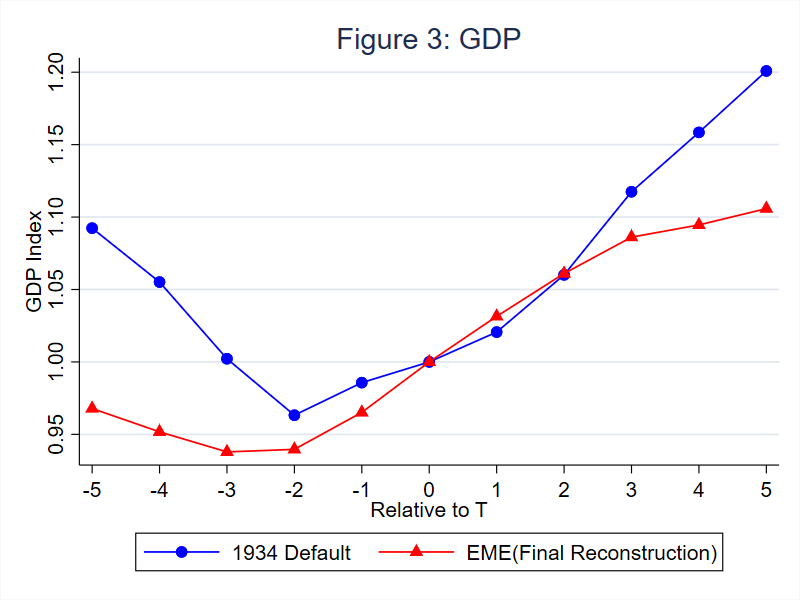
\includegraphics[width=\textwidth]{figures/Figure3_GDP_Comparison.png}
        \caption{Real per capita GDP around debt relief events (exit from default) in middle- to high-
income emerging markets (1978-2010) and advanced economies (1934).}
        \label{fig:3}
    \end{subfigure}
    \hfill
    \begin{subfigure}[b]{0.48\textwidth}
        \centering
        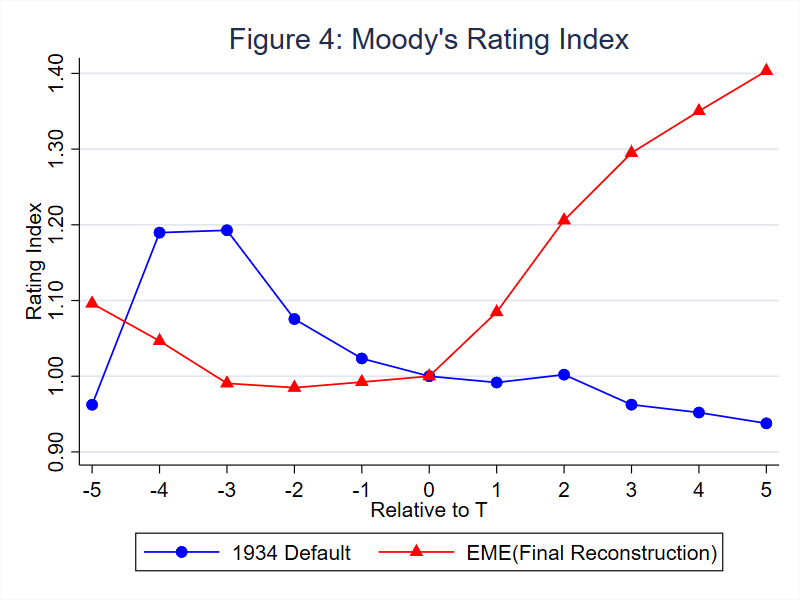
\includegraphics[width=\textwidth]{figures/Figure4_Rating_Comparison.png}
        \caption{Total external debt to GDP (in \%) around debt relief events (exit from default) in
        middle- to high-income emerging markets (1978-2010) and advanced economies (1934).}
        \label{fig:4}
    \end{subfigure}
\end{figure}

\begin{figure}[ht!]
    \centering
    \begin{subfigure}[b]{0.48\textwidth}
        \centering
        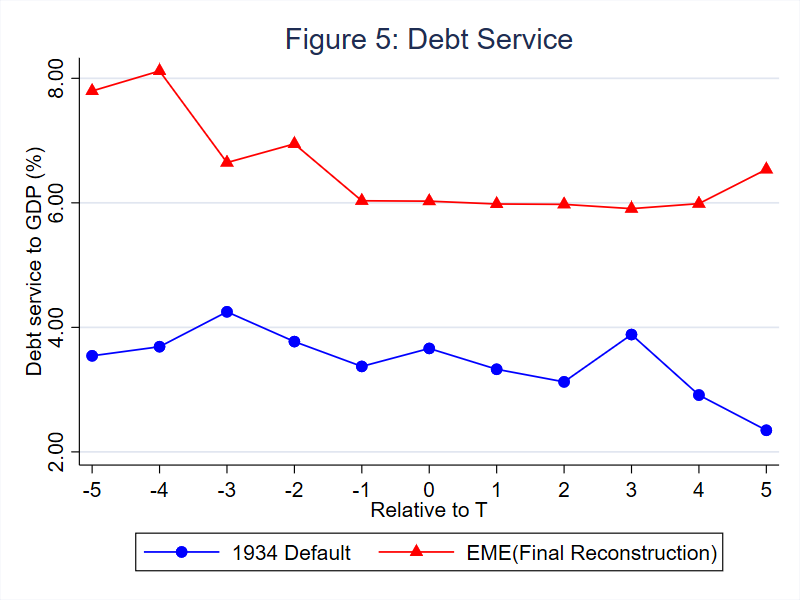
\includegraphics[width=\textwidth]{figures/Figure5_DebtService_Comparison.png}
        \caption{Total debt service to GDP (in \%) around debt relief events (exit from default) in
        middle- to high-income emerging markets (1978-2010) and advanced economies (1934).}
        \label{fig:5}
    \end{subfigure}
    \hfill
    \begin{subfigure}[b]{0.48\textwidth}
        \centering
        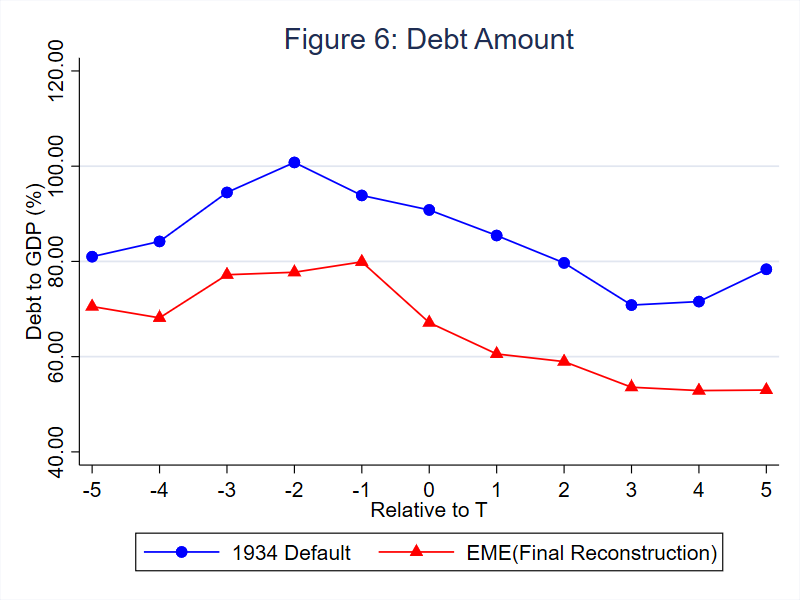
\includegraphics[width=\textwidth]{figures/Figure6_DebtStock_Comparison.png}
        \caption{Debt to GDP (in \%) around debt relief events (exit from default) in middle- to high-
income emerging markets (1978-2010) and advanced economies (1934).}
        \label{fig:6}
    \end{subfigure}
\end{figure}

\subsection{Parallel trend test}
We found out that the author only used the data to make descriptive analysis, but did not
use the data to make a parallel trend test. So, we work on the parallel trend test ourselves, and the results are as below.

To see the results more easily, we write into a matrix:
\begin{table}[ht!]
\centering
\begin{tabular}{lccc}
\toprule
Variable & P‐Value & Pass (5\%) & Pass (10\%) \\
\midrule
GDP\_Growth\_1934\_l   & 0.52529567 & 1 & 1 \\
GDP\_Growth\_1934\_e   & 0.94559858 & 1 & 1 \\
Ratings\_1934          & 0.04996219 & 0 & 0 \\
DebtServ\_1934\_l      & 0.13978740 & 1 & 1 \\
DebtServ\_1934\_e      & 0.51155188 & 1 & 1 \\
Debt\_GDP\_1934\_l     & 0.12776463 & 1 & 1 \\
Debt\_GDP\_1934\_e     & 0.25006164 & 1 & 1 \\
ExtDebt\_1934          & 0.06999843 & 1 & 0 \\
\midrule
GDP\_Growth\_1931\_l   & 0.57373095 & 1 & 1 \\
GDP\_Growth\_1931\_e   & 0.23592213 & 1 & 1 \\
Ratings\_1931          & 0.41062027 & 1 & 1 \\
DebtServ\_1931\_l      & 0.28772333 & 1 & 1 \\
DebtServ\_1931\_e      & 0.39504800 & 1 & 1 \\
Debt\_GDP\_1931\_l     & 0.01403155 & 0 & 0 \\
Debt\_GDP\_1931\_e     & 0.07416818 & 1 & 0 \\
ExtDebt\_1931          & 0.01362215 & 0 & 0 \\
\bottomrule
\end{tabular}
\caption{P-values and pass/fail indicators at 5\% and 10\% levels}
\label{tab:pass_tests}
\end{table}


From this table, we could see that main results are available, most variables pass the test,
only two variables failed, which we need to interpret with caution:
\begin{itemize}
    \item Credit rating results for 1934
    \item Debt/GDP ratio and external debt/GDP ratio results for 1931
\end{itemize}

\begin{figure}[ht!]
    \centering
    \begin{subfigure}[b]{0.48\textwidth}
        \centering
        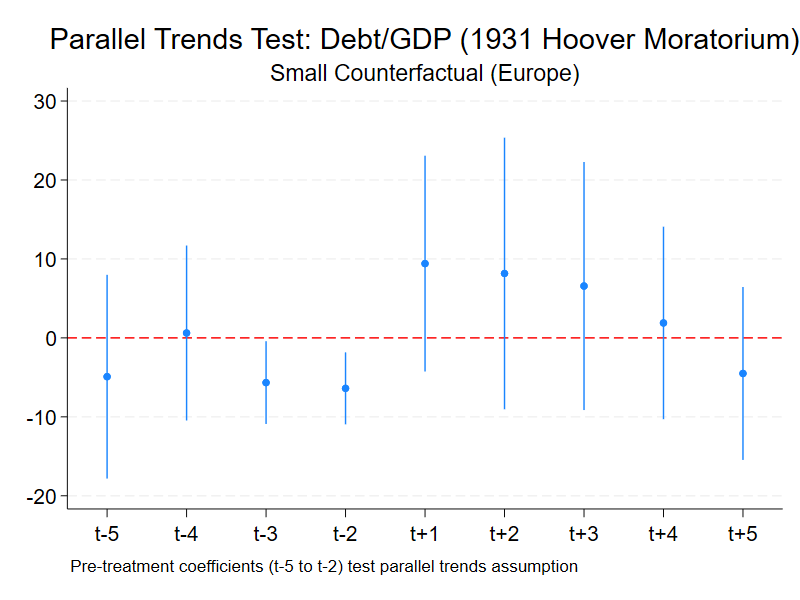
\includegraphics[width=\textwidth]{figures/PT_Debt_1931_Small.png}
        \caption{Parallel Trend Test 1}
        \label{fig:pt1}
    \end{subfigure}
    \hfill
    \begin{subfigure}[b]{0.48\textwidth}
        \centering
        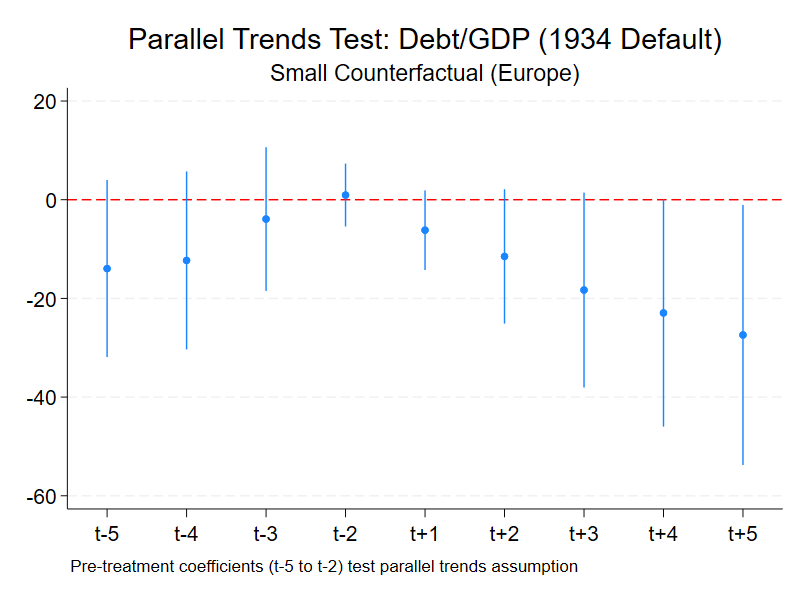
\includegraphics[width=\textwidth]{figures/PT_Debt_1934_Small.png}
        \caption{Parallel Trend Test 2}
        \label{fig:pt2}
    \end{subfigure}
    \\[1em]
    \begin{subfigure}[b]{0.48\textwidth}
        \centering
        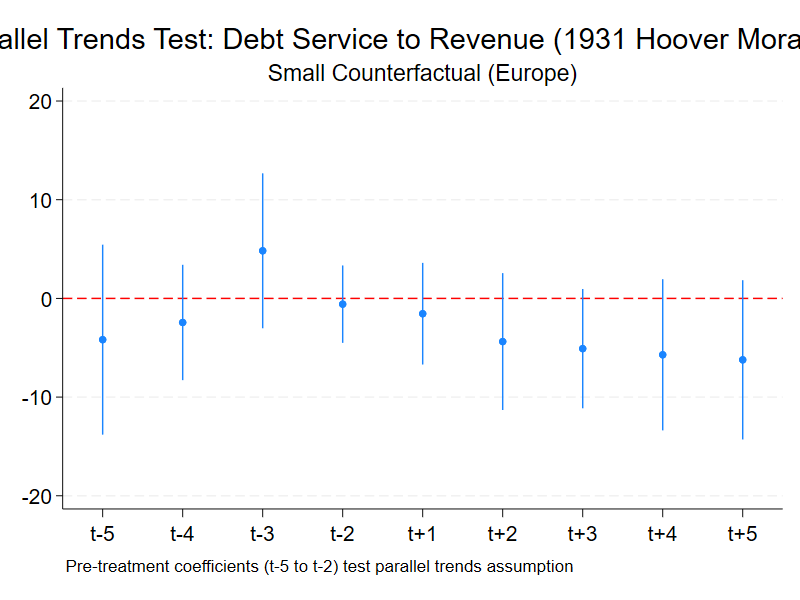
\includegraphics[width=\textwidth]{figures/PT_DebtServ_1931_Small.png}
        \caption{Parallel Trend Test 3}
        \label{fig:pt3}
    \end{subfigure}
    \hfill
    \begin{subfigure}[b]{0.48\textwidth}
        \centering
        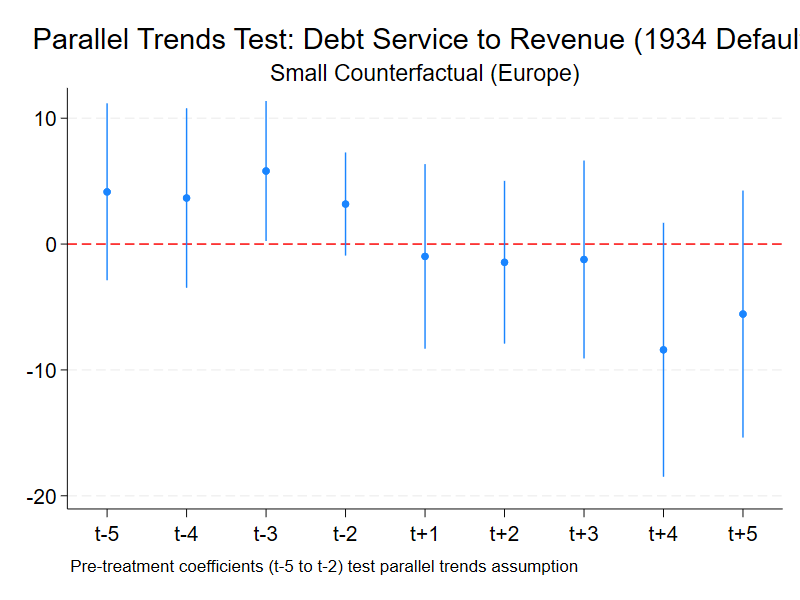
\includegraphics[width=\textwidth]{figures/PT_DebtServ_1934_Small.png}
        \caption{Parallel Trend Test 4}
        \label{fig:pt4}
    \end{subfigure}
    \\[1em]
    \begin{subfigure}[b]{0.48\textwidth}
        \centering
        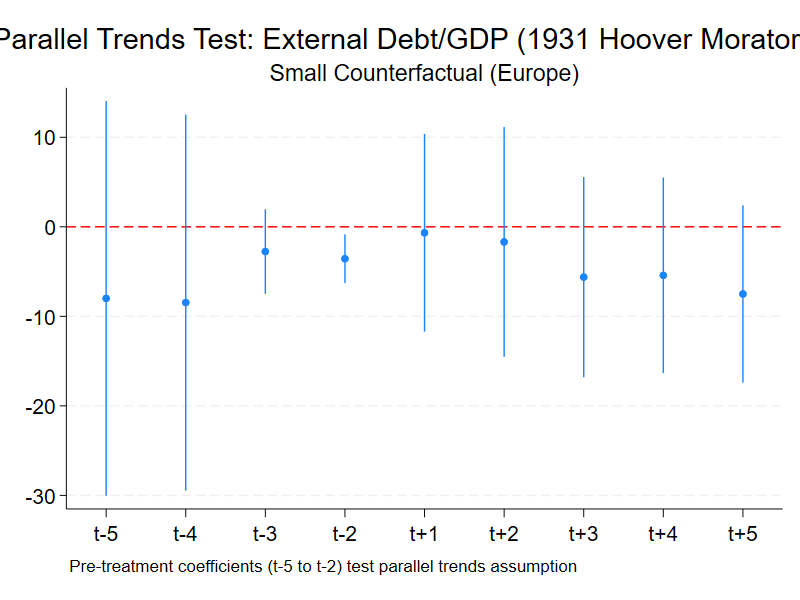
\includegraphics[width=\textwidth]{figures/PT_ExtDebt_1931.png}
        \caption{Parallel Trend Test 5}
        \label{fig:pt5}
    \end{subfigure}
    \hfill
    \begin{subfigure}[b]{0.48\textwidth}
        \centering
        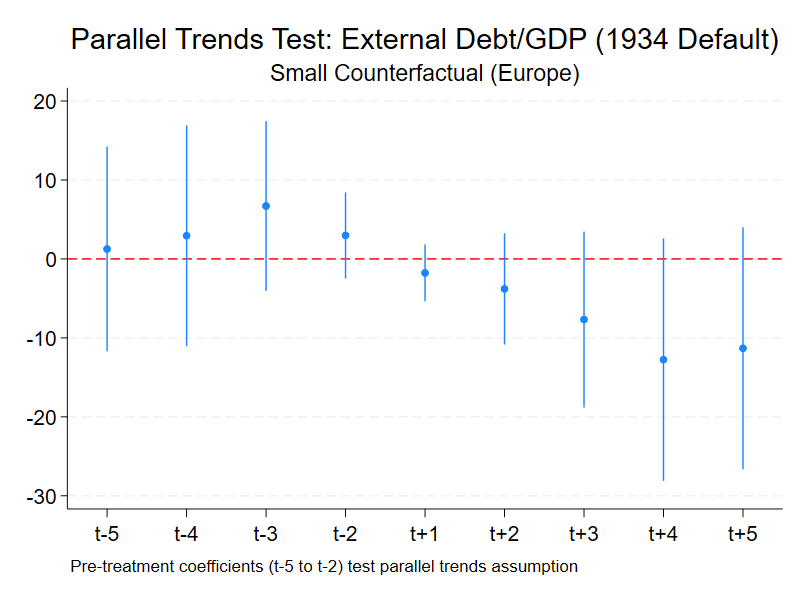
\includegraphics[width=\textwidth]{figures/PT_ExtDebt_1934.png}
        \caption{Parallel Trend Test 6}
        \label{fig:pt6}
    \end{subfigure}
    \\[1em]
    \begin{subfigure}[b]{0.48\textwidth}
        \centering
        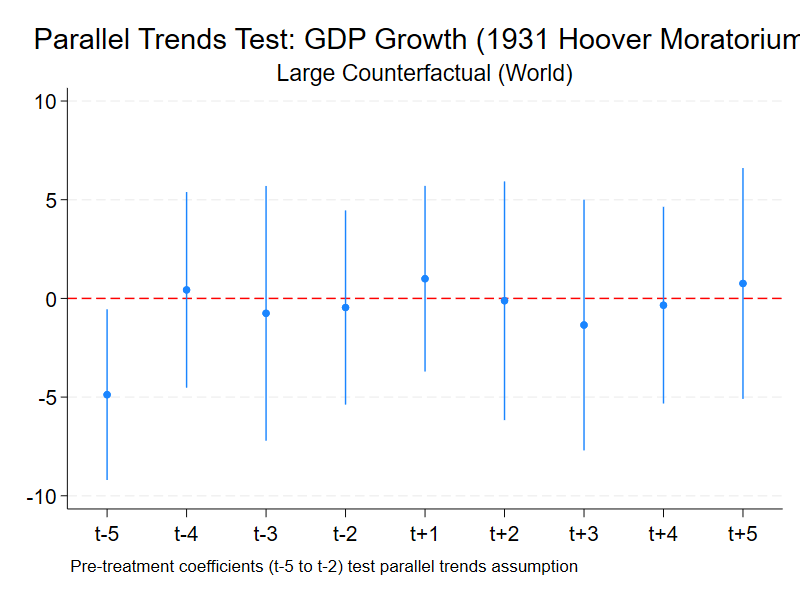
\includegraphics[width=\textwidth]{figures/PT_GDP_1931_Large.png}
        \caption{Parallel Trend Test 7}
        \label{fig:pt7}
    \end{subfigure}
    \hfill
    \begin{subfigure}[b]{0.48\textwidth}
        \centering
        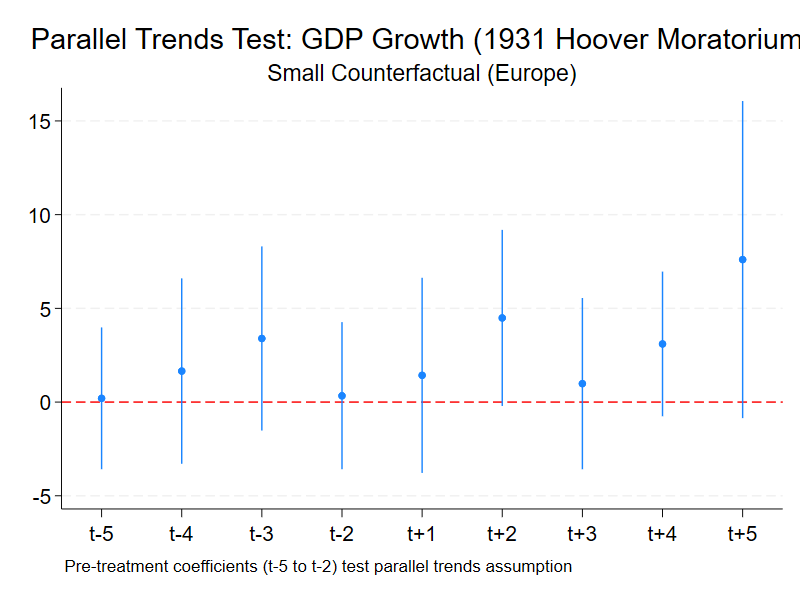
\includegraphics[width=\textwidth]{figures/PT_GDP_1931_Small.png}
        \caption{Parallel Trend Test 8}
        \label{fig:pt8}
    \end{subfigure}
    \caption{Parallel trend test results for different country samples and variables}
    \label{fig:parallel_trends}
\end{figure}

\begin{figure}[ht!]
    \centering
    \begin{subfigure}[b]{0.48\textwidth}
        \centering
        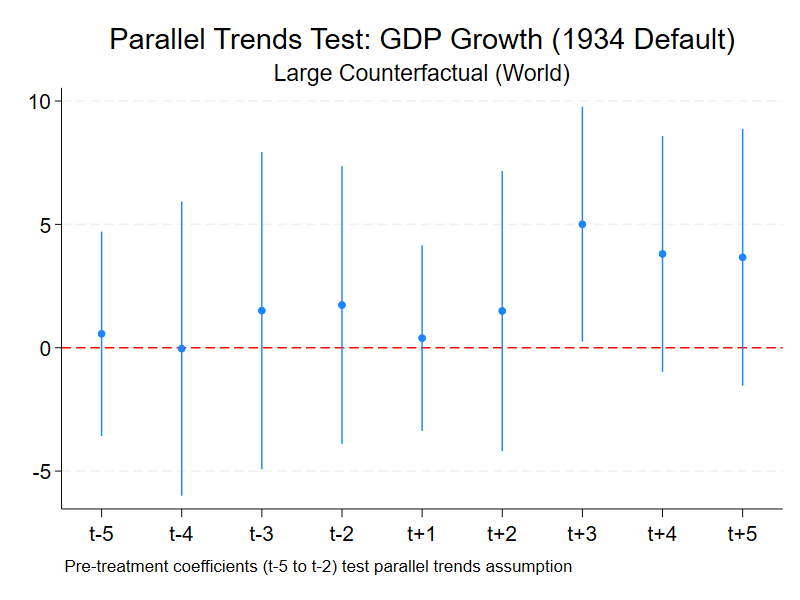
\includegraphics[width=\textwidth]{figures/PT_GDP_1934_Large.png}
        \caption{Parallel Trend Test 9}
        \label{fig:pt9}
    \end{subfigure}
    \hfill
    \begin{subfigure}[b]{0.48\textwidth}
        \centering
        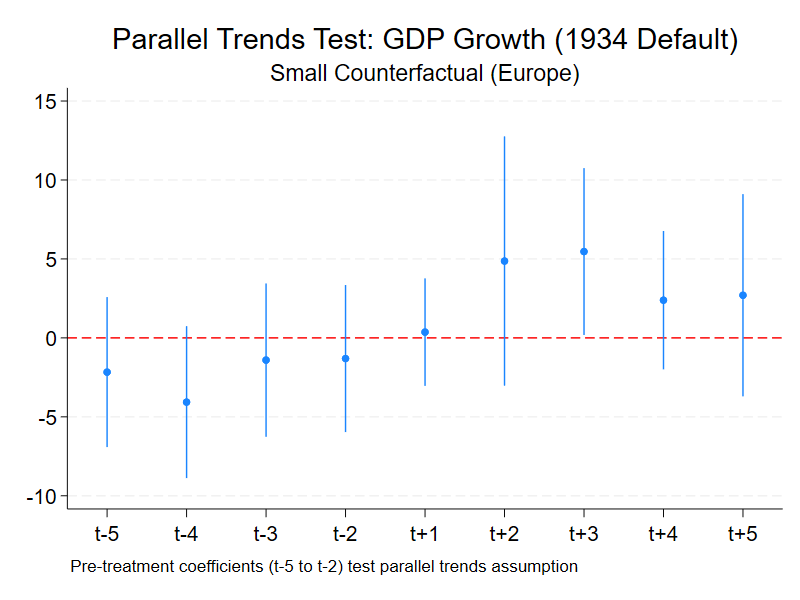
\includegraphics[width=\textwidth]{figures/PT_GDP_1934_Small.png}
        \caption{Parallel Trend Test 10}
        \label{fig:pt10}
    \end{subfigure}
    \hfill
    \begin{subfigure}[b]{0.48\textwidth}
        \centering
        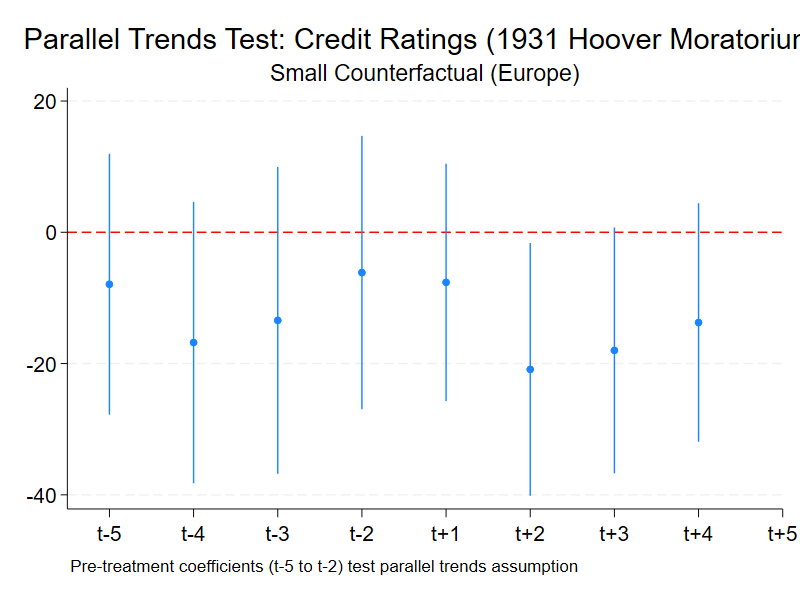
\includegraphics[width=\textwidth]{figures/PT_Ratings_1931.png}
        \caption{Parallel Trend Test 11}
        \label{fig:pt11}
    \end{subfigure}
    \hfill
    \begin{subfigure}[b]{0.48\textwidth}
        \centering
        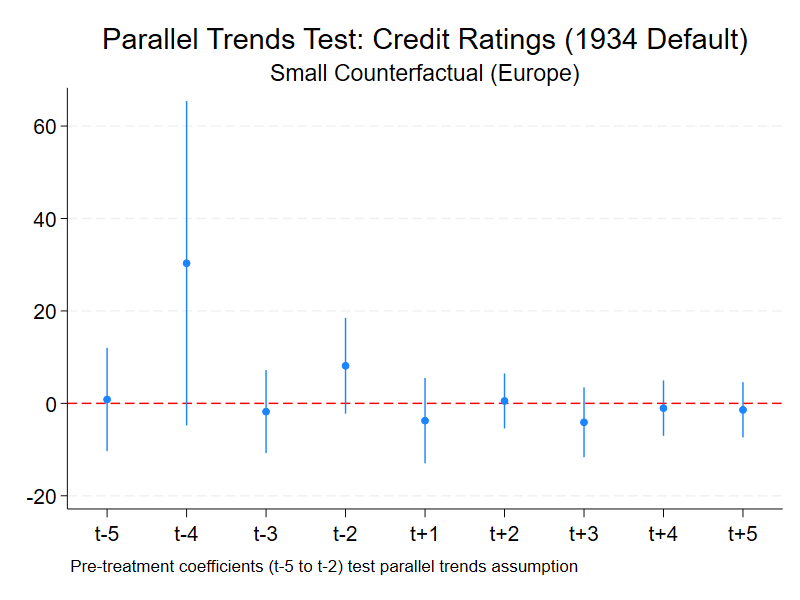
\includegraphics[width=\textwidth]{figures/PT_Ratings_1934.png}
        \caption{Parallel Trend Test 12}
        \label{fig:pt12}
    \end{subfigure}
    \caption{Parallel trend test results for different country samples and variables}
    \label{fig:parallel_trends2}
\end{figure}

\subsection{DID Analysis}

The Brady target group includes all middle-income
EMs with a Brady deal, namely Argentina, Brazil, Bulgaria, Costa Rica, Dominican
Republic, Ecuador, Jordan, Mexico, Panama, Peru, Poland, Uruguay, and Venezuela.
The Baker country sample is the same, plus Chile, which was a target country in the
mid-1980s, but were not part of the “Brady bunch”.

The baseline counterfactual includes all middle- and high-income countries(regions)
that did not default nor received debt relief in this period and for which we have data,
namely China, Colombia, Czech Republic, Egypt, Hungary, India, Israel, Malaysia,
Mauritius, Singapore, South Korea, Taiwan, Thailand, and Turkey.

We start with the Hoover Moratorium of 1931 and take a preliminary view of the
data.

\begin{figure}[ht!]
    \centering
    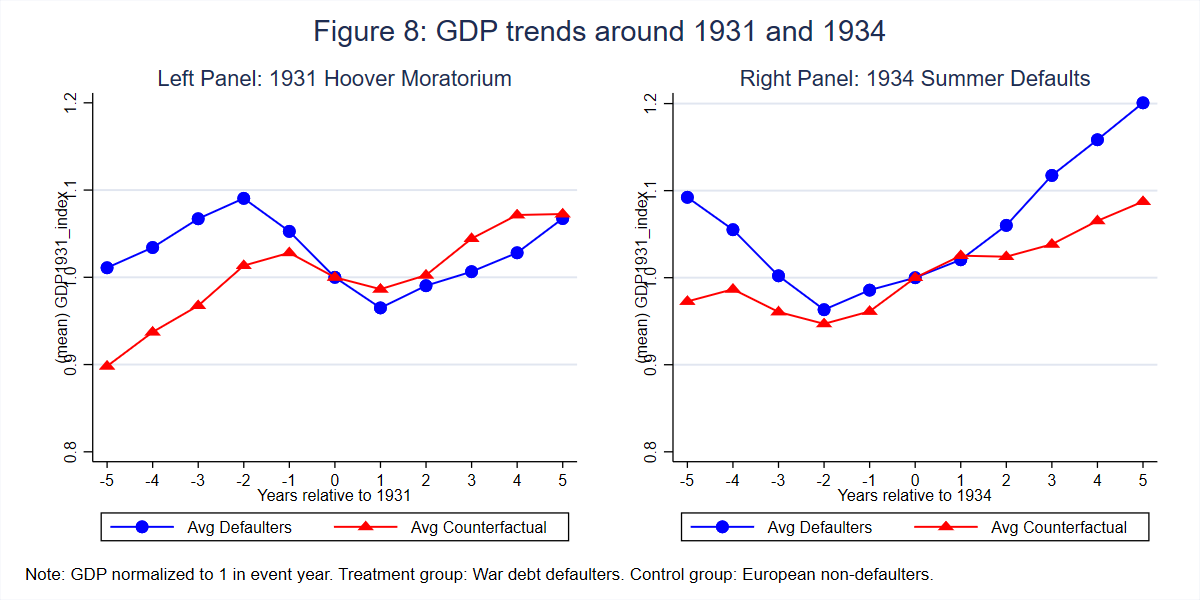
\includegraphics[width=0.95\textwidth]{figures/Figure8_GDP_trends_1931_1934.png}
    \caption{GDP trends around 1931 and 1934}
    \label{fig:8}
\end{figure}

\begin{figure}[ht!]
    \centering
    \begin{subfigure}[b]{0.48\textwidth}
        \centering
        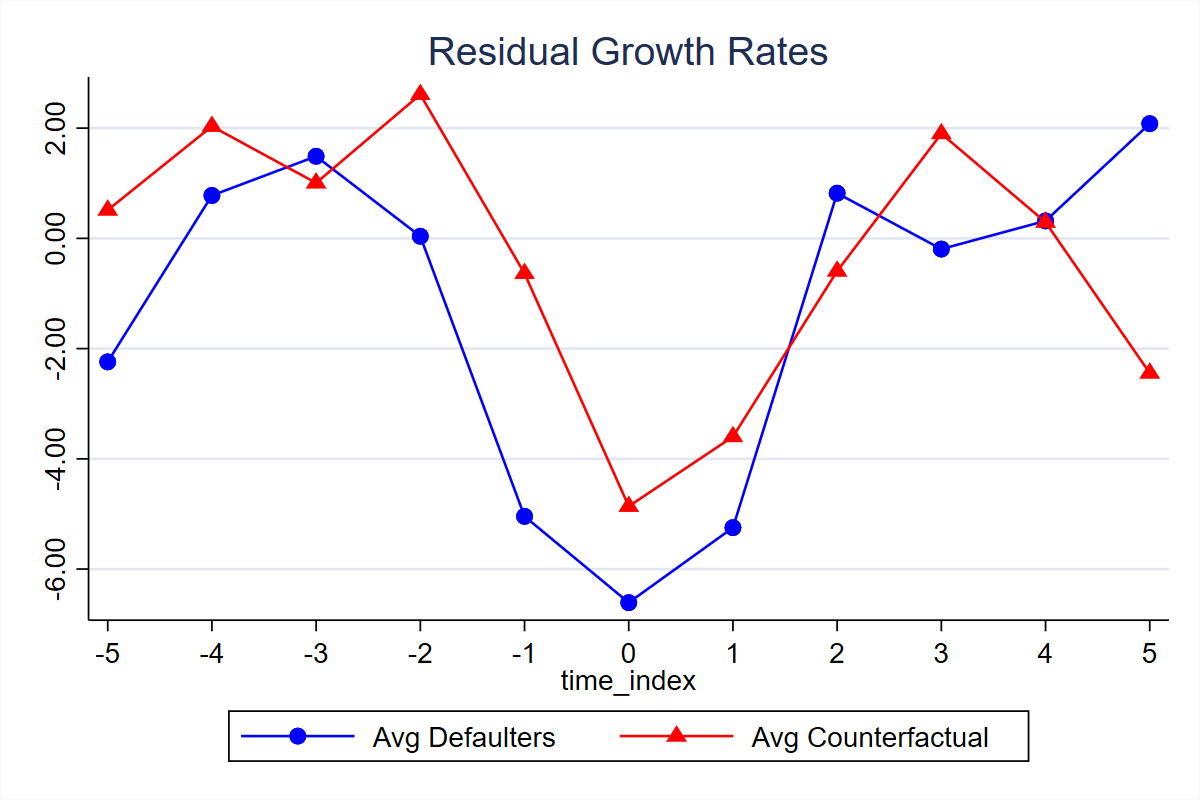
\includegraphics[width=\textwidth]{figures/figc5_a.png}
        \caption{Residual GDP Growth}
        \label{fig:c5a}
    \end{subfigure}
    \hfill
    \begin{subfigure}[b]{0.48\textwidth}
        \centering
        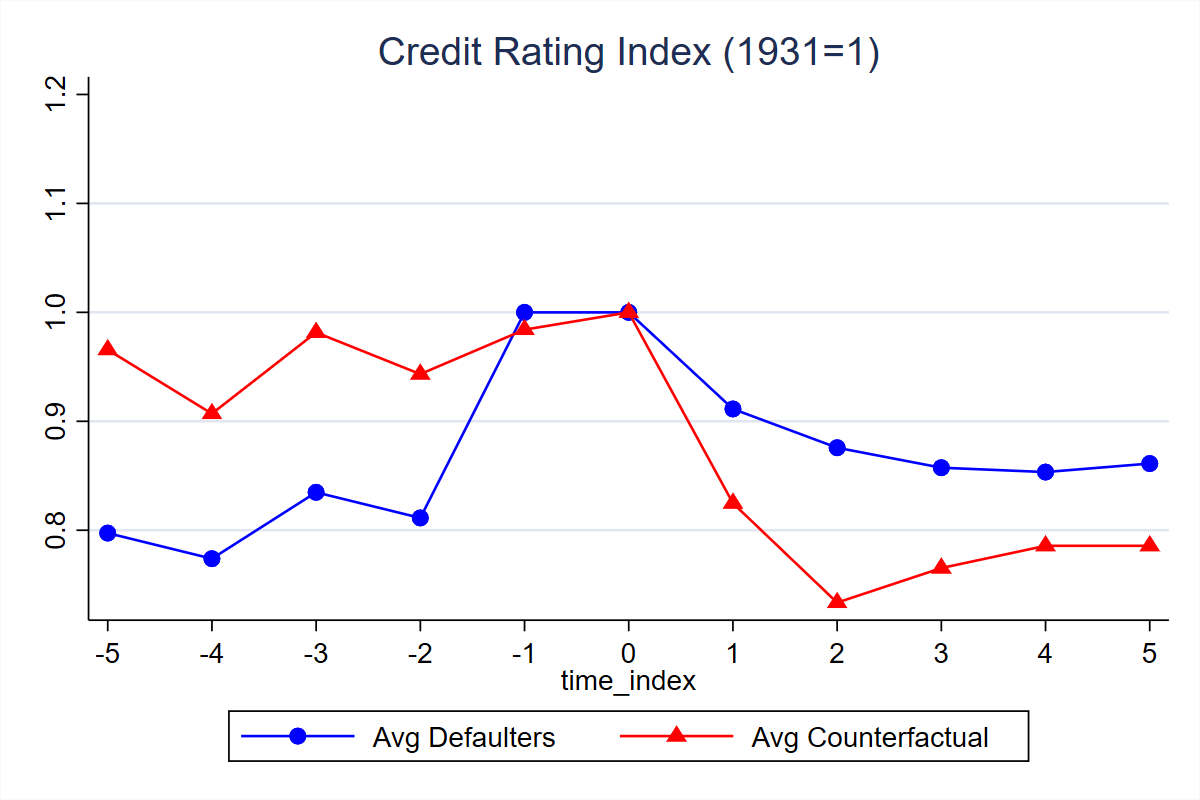
\includegraphics[width=\textwidth]{figures/figc5_b.png}
        \caption{Credit Ratings}
        \label{fig:c5b}
    \end{subfigure}
    \\[1em]
    \begin{subfigure}[b]{0.48\textwidth}
        \centering
        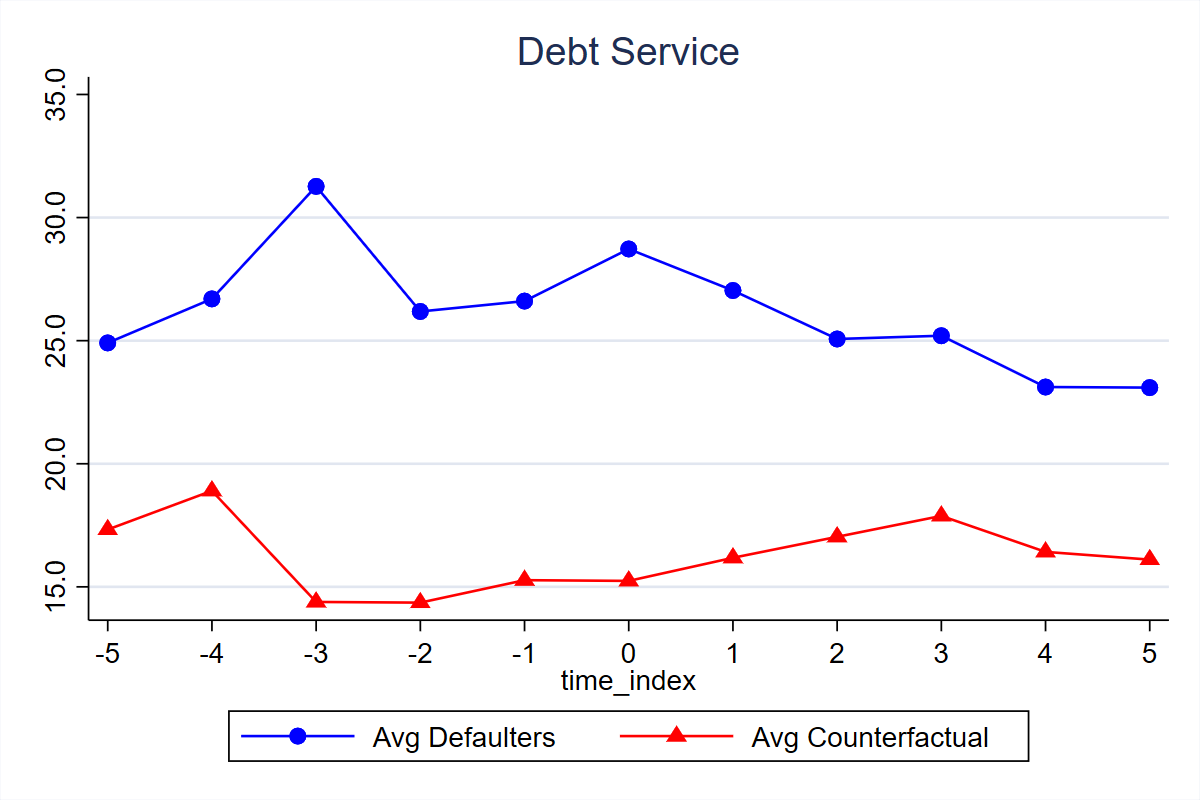
\includegraphics[width=\textwidth]{figures/figc5_c.png}
        \caption{Debt Service to Revenue}
        \label{fig:c5c}
    \end{subfigure}
    \hfill
    \begin{subfigure}[b]{0.48\textwidth}
        \centering
        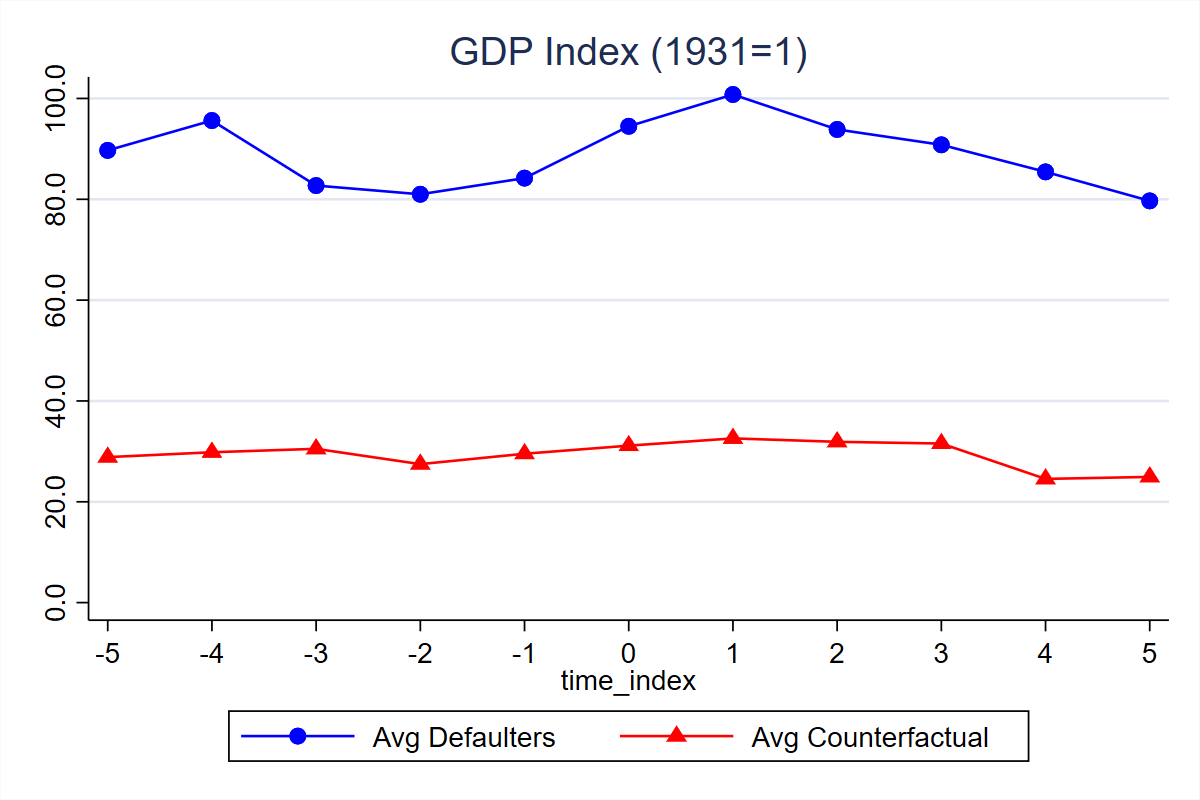
\includegraphics[width=\textwidth]{figures/figc5_d.png}
        \caption{Debt to GDP}
        \label{fig:c5d}
    \end{subfigure}
    \caption{Economic indicators comparison between treatment and control groups}
    \label{fig:c5}
\end{figure}

The figures compare the development of our main economic indicators for treatment and control groups,
where the control groups is our baseline sample of European non-defaulters.
Figure 8 (left panel) shows that the growth performance of the treatment group is significantly worse
than that of the counterfactual around 1931. 

Panel B: country
heterogeneity by showing residuals from a regression of annual real p.c. growth on a
constant and country-specific dummies. Residual growth declines markedly for both
groups prior to 1931 and recovers strongly afterwards, but there is no evidence that
treatment countries perform better than the counterfactual.

Panel C: The picture is similarly
bleak with regard to Moody's credit ratings, which decline across the board after 1931,
with no notable difference between the two groups. 

Panel D: Similarly, the debt/GDP
level does not decline significantly more for the target countries. Only the
debt servicing burden improves, as payments to revenue drop relatively more than
those countries not receiving relief.

\subsection{Results of DID}
The results are more notable for the 1934 debt relief spell. Table 4 indicates that
real per capita growth is 4.7 percentage points higher for treated countries in the post-
1934 period, with a highly significant coefficient (column (1)). Moreover, the debt
levels decrease significantly (columns (6) and (8)), compared to the counterfactual on
European non-defaulters. We find no significant coefficient for debt servicing (column
(4)) and a highly significant negative coefficient for ratings. These results, however,
are rather sensitive to the choice of counterfactual, as can be seen in columns (2),
(5), and (7), which use the “World” counterfactual including European, Asian, and
South American countries. The treatment coefficient for debt servicing becomes highly
significant and large, while the coefficient for debt/GDP turns insignificant. Notably,
however, the growth coefficient remains large and significant across all counterfactuals
chosen, albeit sometimes only at the 10\% level.

\begin{sidewaystable}[ht!]\centering
\def\sym#1{\ifmmode^{#1}\else\(^{#1}\)\fi}
\caption{Table 3: 1931 Hoover Moratorium - Difference-in-Difference Analysis}
\renewcommand{\arraystretch}{1.2} % 增加行距
\begin{tabular*}{\textwidth}{@{\hskip\tabcolsep\extracolsep\fill}p{3.75cm}*{8}{>{\centering\arraybackslash}p{2.25cm}}}
\hline\hline
            &(1)&(2)&(3)&(4)&(5)&(6)&(7)&(8)\\
            &\parbox{2.25cm}{\centering Growth, real p.c.\\Small (Europe)}&\parbox{2.25cm}{\centering Growth, real p.c.\\Large (World)}&\parbox{2.25cm}{\centering Credit Ratings (change)\\Small (Europe)}&\parbox{2.25cm}{\centering Debt Service to Revenue\\Small (Europe)}&\parbox{2.25cm}{\centering Debt Service to Revenue\\Large (World)}&\parbox{2.25cm}{\centering Total Public Debt/GDP\\Small (Europe)}&\parbox{2.25cm}{\centering Total Public Debt/GDP\\Large (World)}&\parbox{2.25cm}{\centering External Debt/GDP\\Small (Europe)}\\
\hline
\parbox{3cm}{\raggedright Post-intervention dummy (after 1931)}&  $4.922^{**}$  &  $8.329^{***}$  &  $3.752$  &  $-1.064$  &  $-3.882^{**}$&  $-10.011^{*}$  &  $-7.900^{*}$ &  $-9.086^{**}$  \\
            &  $(2.335)$  &  $(1.724)$ & $(3.377)$   &  $(1.880)$   &  $(1.854)$  &  $(4.854)$  &  $(4.240)$  & $(3.687)$   \\
[0.5em]
\parbox{3cm}{\raggedright Treatment (war debt moratorium) $\times$ post-intervention dummy}&  $2.598^{*}$&  $0.862$  &  $-5.655$&  $-4.310^{*}$  &  $-3.390$   &  $7.312$ &  $3.822$   &  $-0.508$ \\
            &  $(1.360)$   &  $(1.333)$   &  $(4.202)$   &  $(2.392)$   &  $(2.335)$   &  $(6.936)$   &  $(6.899)$   &  $(5.610)$   \\
[0.5em]
Constant    &  $-4.072^{***}$&  $-4.489^{***}$&  $0.906$   &  $24.360^{***}$&  $23.973^{***}$&  $69.849^{***}$&  $61.471^{***}$&  $32.183^{***}$\\
            &  $(0.839)$   &  $(1.160)$   &  $(2.058)$   &  $(1.215)$   &  $(0.990)$   &  $(1.872)$   &  $(1.695)$   &  $(2.174)$   \\
\hline
Observations&         237   &         373   &         230   &         223   &         326   &         172   &         248   &         167   \\
Adjusted R² &       0.237   &       0.206   &       0.185   &       0.043   &       0.062   &       0.166   &       0.199   &       0.007   \\
\hline\hline
\multicolumn{9}{p{0.95\textwidth}}{\footnotesize \textbf{Notes:} This table reports difference-in-difference estimates of the effect of the 1931 Hoover Moratorium on various economic outcomes. Treatment group consists of 18 countries that received war debt relief. Small counterfactual includes European non-defaulters; Large counterfactual adds Latin American and other countries. All regressions include country and year fixed effects. Standard errors clustered at country level in parentheses. $^*$ p<0.10, $^{**}$ p<0.05, $^{***}$ p<0.01}\\
\end{tabular*}
\end{sidewaystable}


When we are working on Table3, we found out a bug:
the data of column (3), (4), (5) might be in the wrong order, the correct order of data should be (5), (3), (4).

Also, the post-intervention dummy (after 1931) is very different from authors' result, we also tried to drop the year fixed effect, but the result is still different.
(We tried to run authors' original code, and the results are the same as what we get, not what's in the table of this paper.)

According to the authors based on their result, `The only $\beta_2$ coefficients that are marginally significant are those of GDP and of credit ratings',
but as we could see from our table, only credit ratings and debt service to revenue in treated countries are insignificant.

\begin{figure}[ht!]
    \centering
    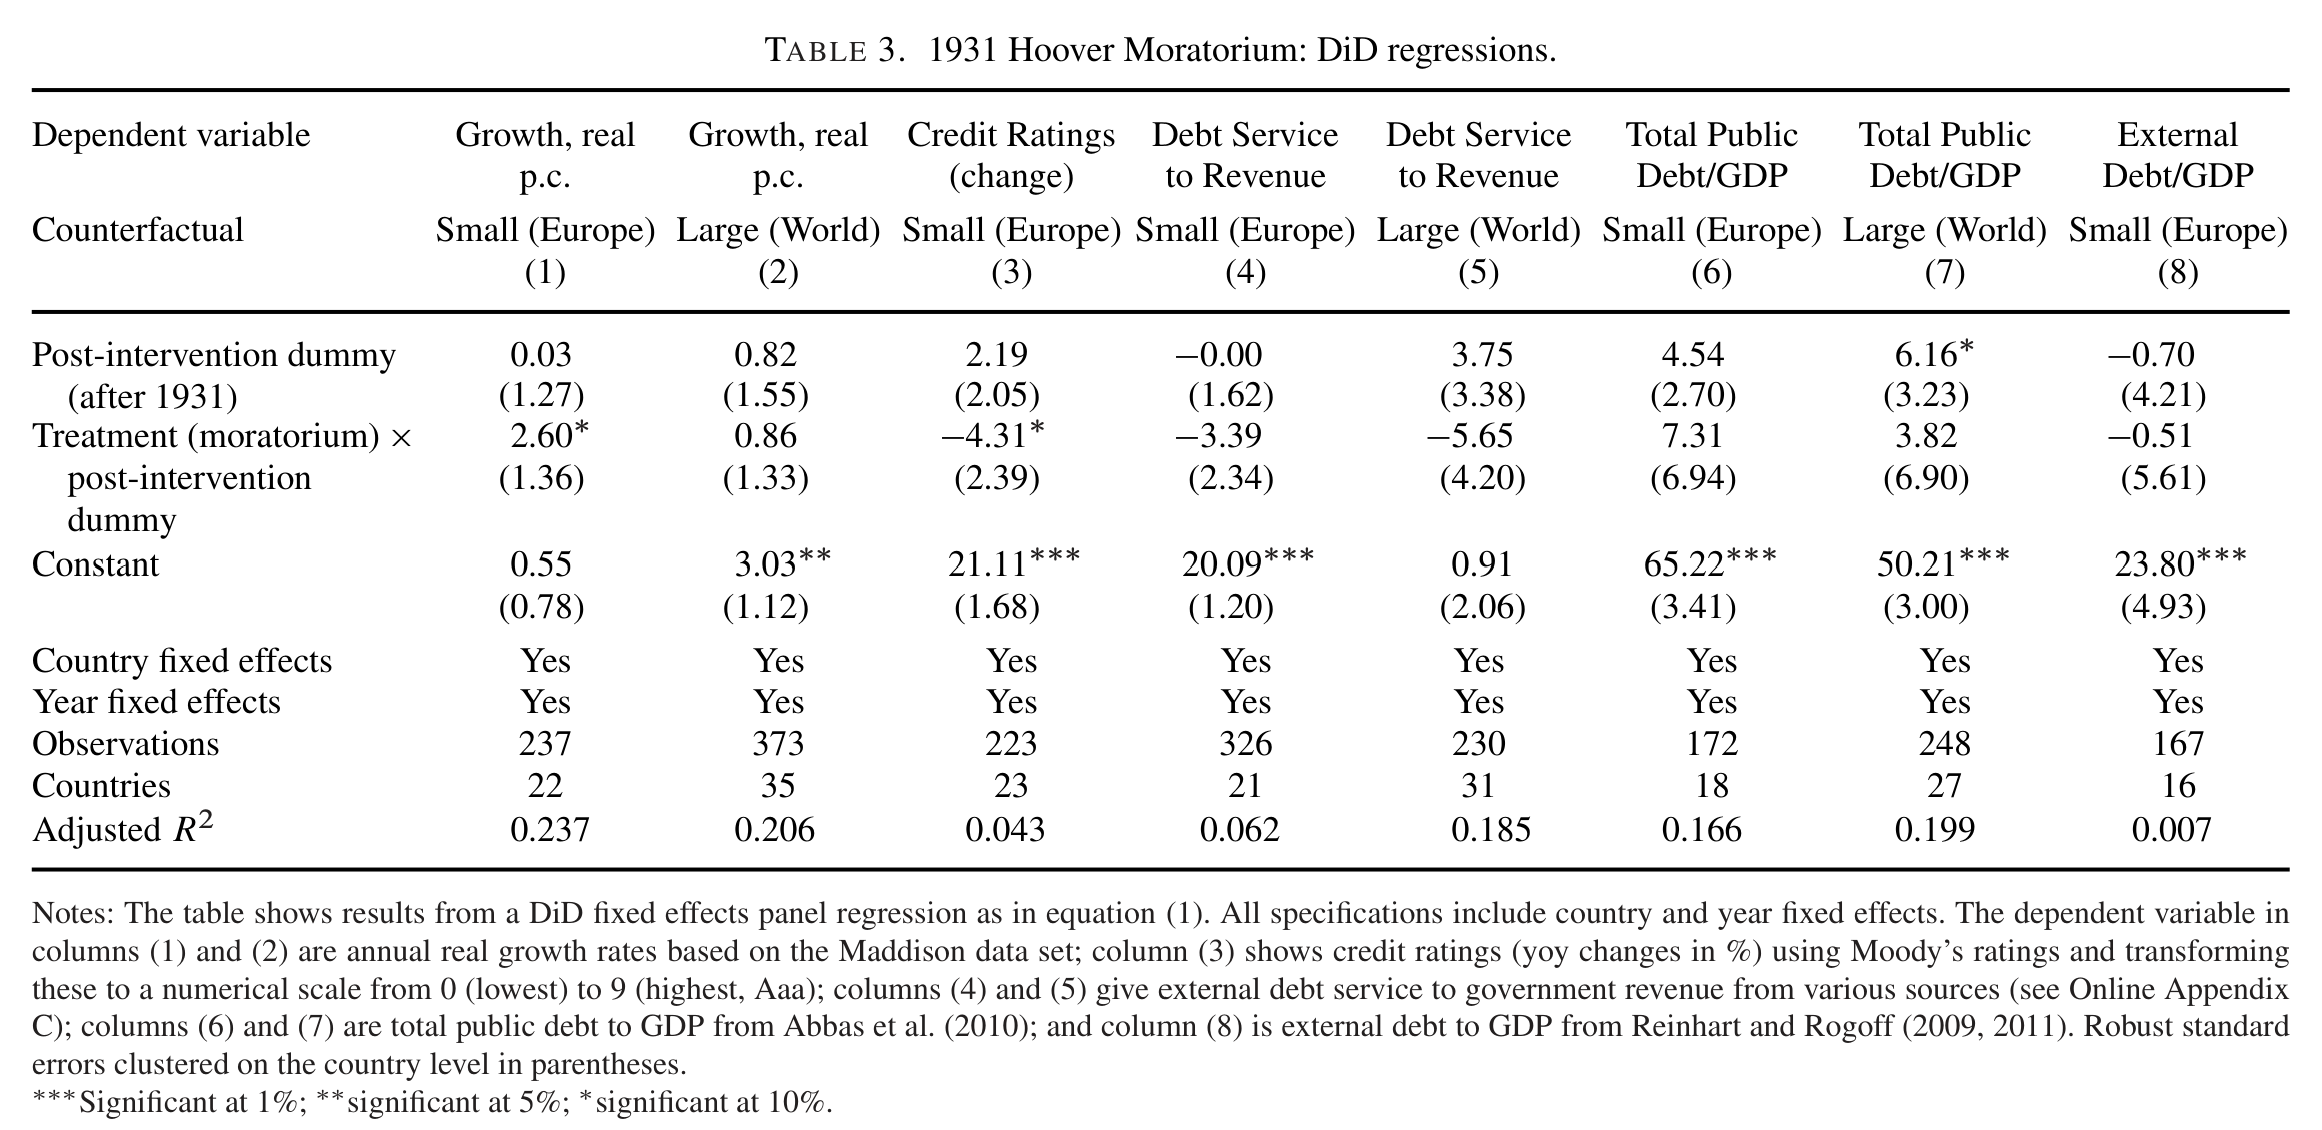
\includegraphics[width=0.95\textwidth]{figures/table3_original.png}
    \caption{Table 3 Original}
    \label{fig:table3_original}
\end{figure}

\begin{figure}[ht!]
    \centering
    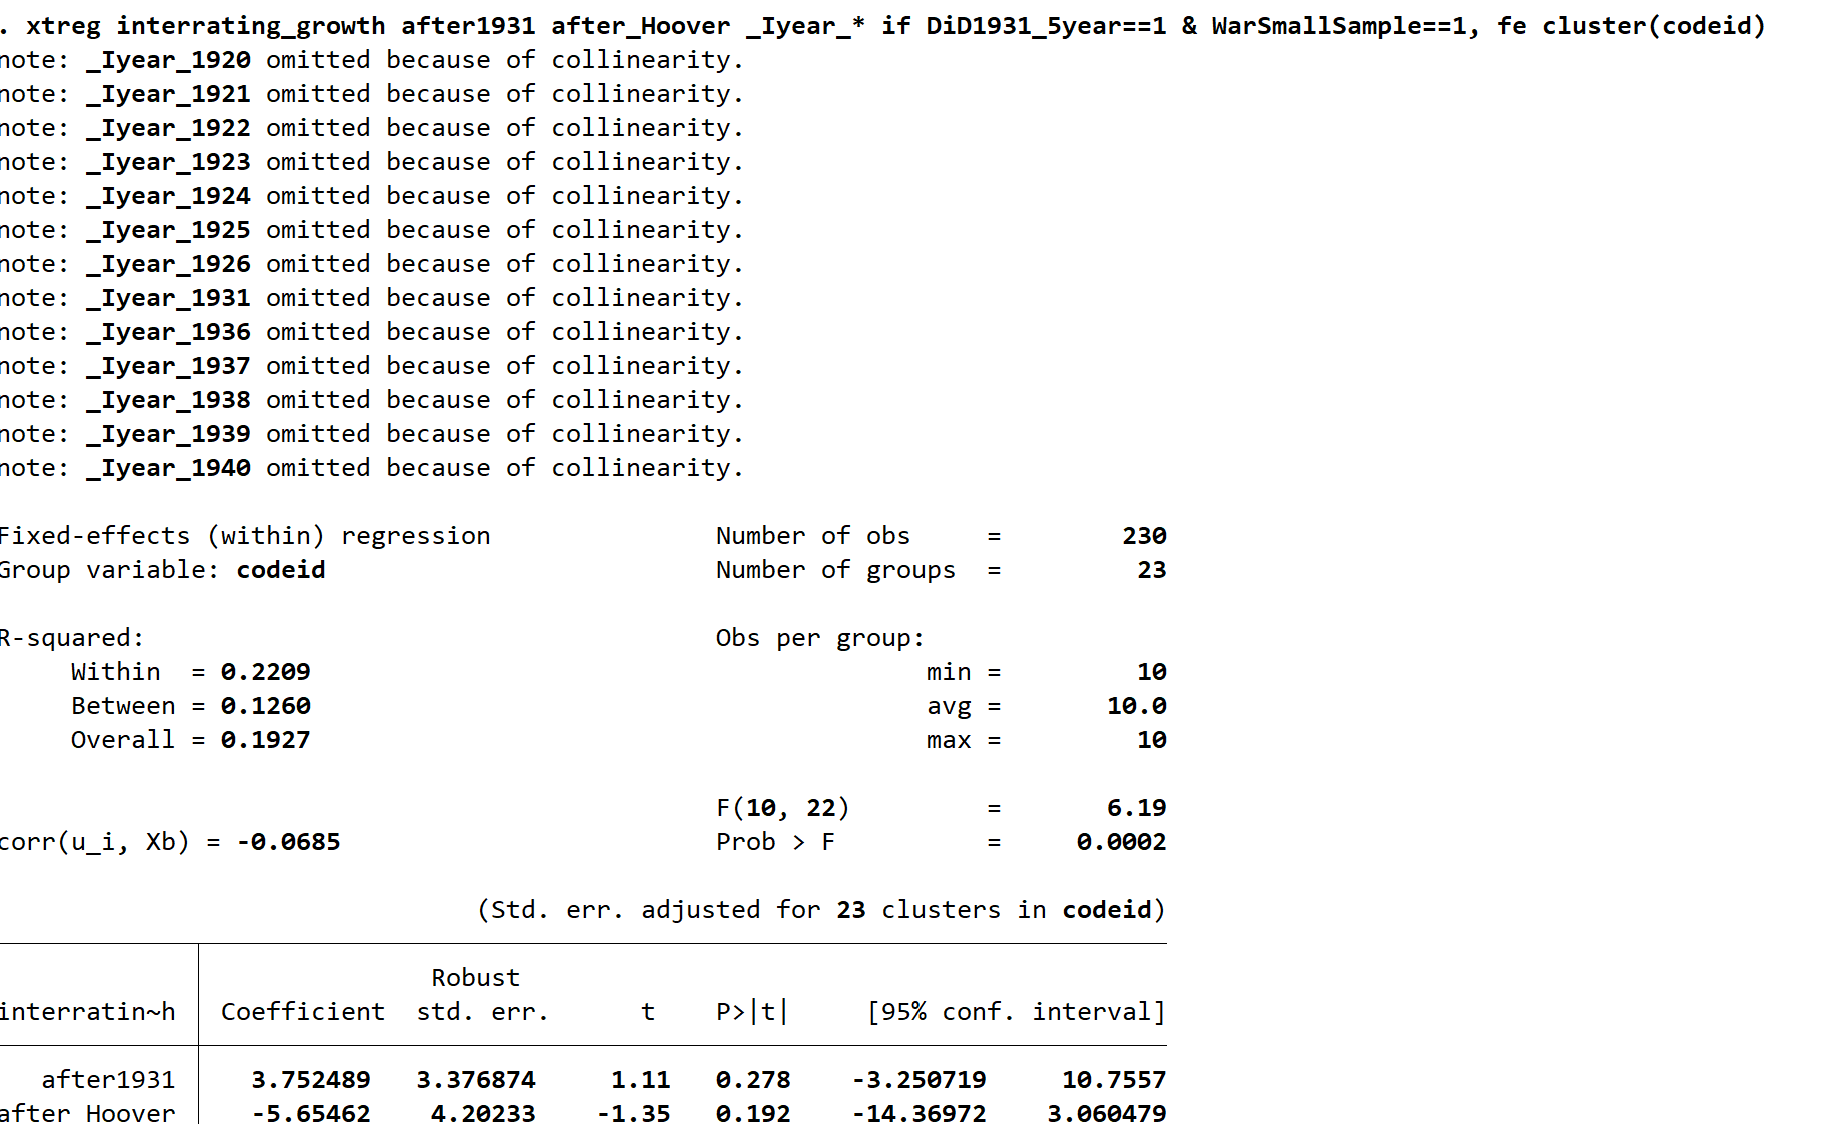
\includegraphics[width=0.95\textwidth]{figures/col3_tab3_stata.png}
    \caption{Table 3 Col 3}
    \label{fig:table3_col3}
\end{figure}

\begin{figure}[ht!]
    \centering
    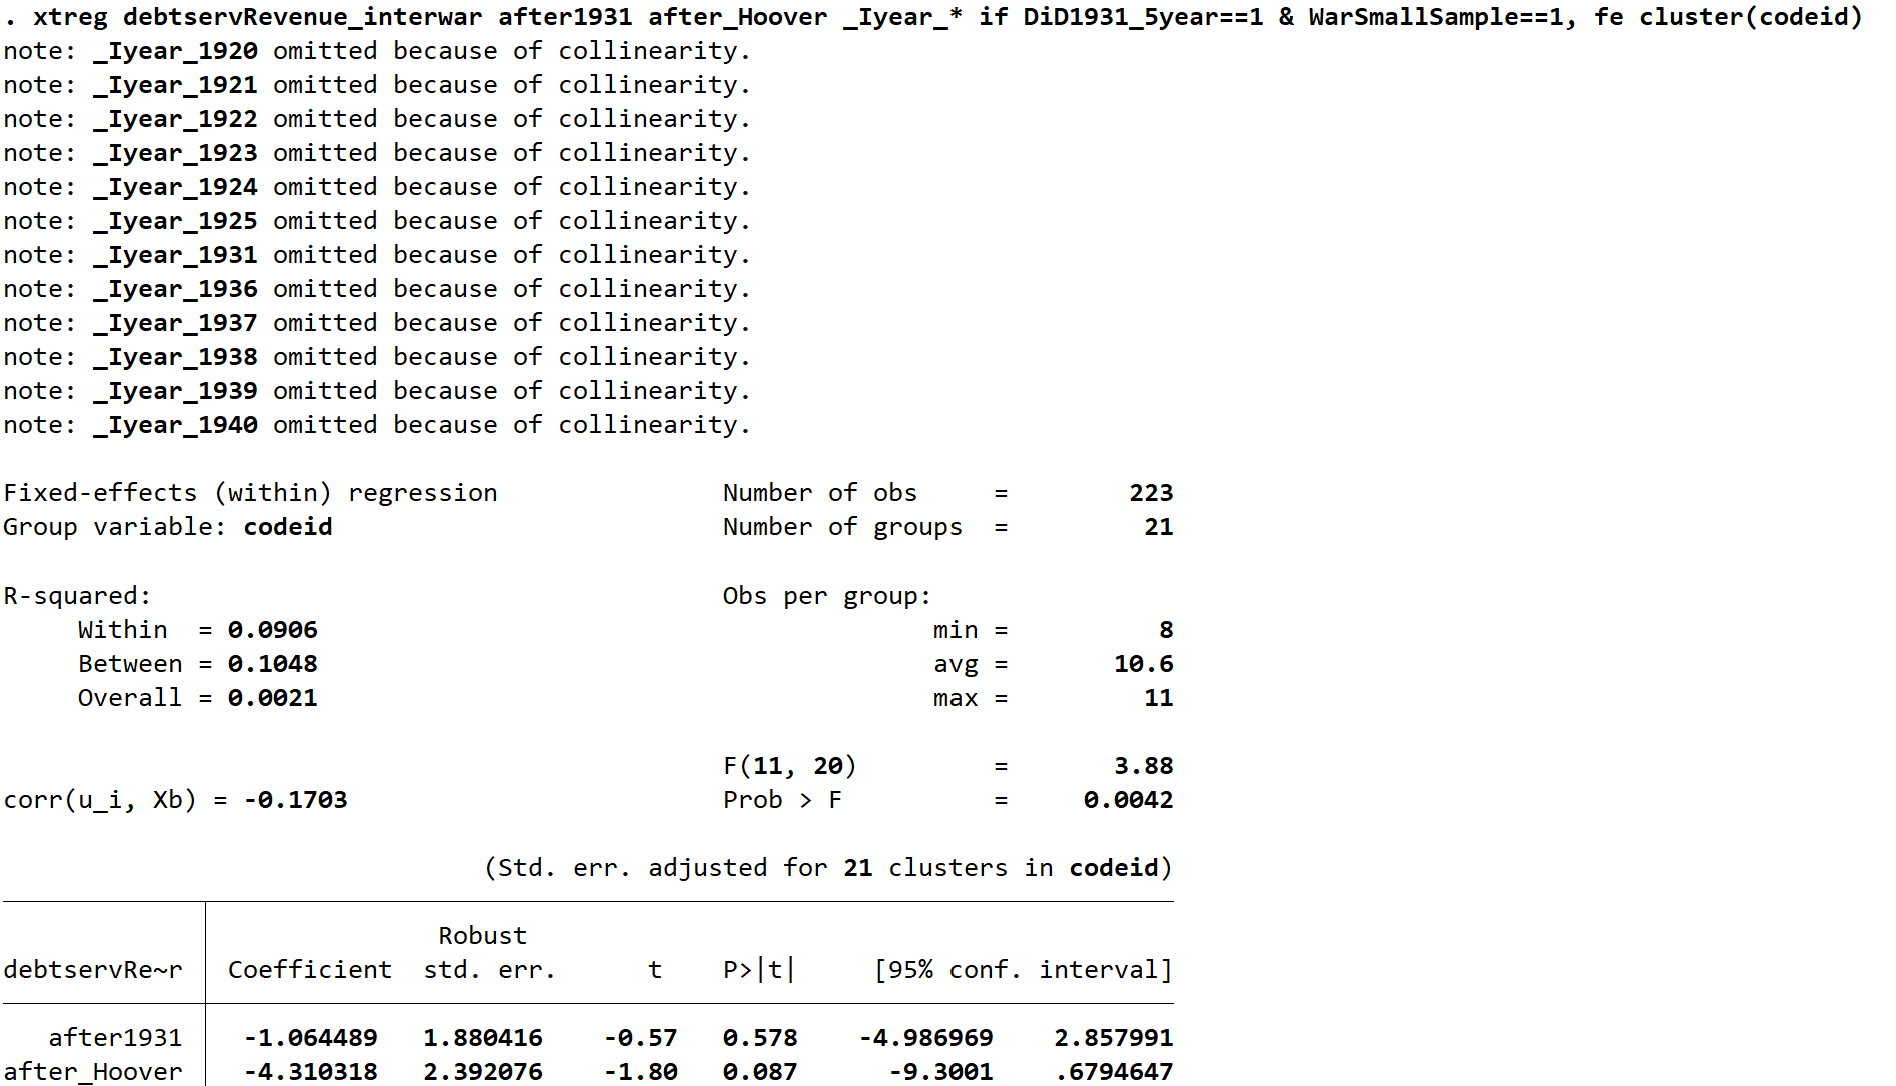
\includegraphics[width=0.95\textwidth]{figures/col4_tab3_stata.png}
    \caption{Table 3 Col 4}
    \label{fig:table3_col4}
\end{figure}

\begin{sidewaystable}[ht!]\centering
\def\sym#1{\ifmmode^{#1}\else\(^{#1}\)\fi}
\caption{Table 4: 1934 Summer Defaults - Difference-in-Difference Analysis}
\renewcommand{\arraystretch}{1.2} % 增加行距
\begin{tabular*}{\textwidth}{@{\hskip\tabcolsep\extracolsep\fill}p{3.75cm}*{8}{>{\centering\arraybackslash}p{2.25cm}}}
\hline\hline
            &(1)&(2)&(3)&(4)&(5)&(6)&(7)&(8)\\
            &\parbox{2.25cm}{\centering Growth, real p.c.\\Small (Europe)}&\parbox{2.25cm}{\centering Growth, real p.c.\\Large (World)}&\parbox{2.25cm}{\centering Credit Ratings (change)\\Small (Europe)}&\parbox{2.25cm}{\centering Debt Service to Revenue\\Small (Europe)}&\parbox{2.25cm}{\centering Debt Service to Revenue\\Large (World)}&\parbox{2.25cm}{\centering Total Public Debt/GDP\\Small (Europe)}&\parbox{2.25cm}{\centering Total Public Debt/GDP\\Large (World)}&\parbox{2.25cm}{\centering External Debt/GDP\\Small (Europe)}\\
\hline
\parbox{3cm}{\raggedright Post-intervention dummy (after 1934)}&  $-1.905$  &  $-0.772$  &  $4.527^*$  &  $-4.284$  &  $-5.094^{***}$&  $-9.030$  &  $-9.602^{**}$ &  $-3.487$  \\
            &  $(1.320)$  &  $(1.398)$ & $(2.601)$   &  $(2.789)$   &  $(1.837)$  &  $(5.566)$  &  $(4.246)$  & $(3.260)$   \\
[0.5em]
\parbox{3cm}{\raggedright Treatment (debt relief) $\times$ post-intervention dummy}&  $4.658^{***}$&  $2.208^*$  &  $-8.182^{***}$&  $-6.025^*$  &  $-2.744$   &  $-12.206^{**}$ &  $-7.932$   &  $-9.512^{**}$ \\
            &  $(1.437)$   &  $(1.245)$   &  $(2.664)$   &  $(2.989)$   &  $(2.926)$   &  $(5.666)$   &  $(6.180)$   &  $(3.835)$   \\
[0.5em]
Constant    &  $2.399^{***}$&  $3.148^{***}$&  $0.247$   &  $23.094^{***}$&  $21.260^{***}$&  $69.716^{***}$&  $59.571^{***}$&  $25.866^{***}$\\
            &  $(0.643)$   &  $(1.056)$   &  $(2.176)$   &  $(0.950)$   &  $(0.786)$   &  $(3.166)$   &  $(2.382)$   &  $(1.746)$   \\
\hline
Observations&         237   &         378   &         249   &         216   &         324   &         175   &         258   &         162   \\
Adjusted R² &       0.270   &       0.226   &       0.199   &       0.167   &       0.153   &       0.283   &       0.243   &       0.342   \\
\hline\hline
\multicolumn{9}{p{0.95\textwidth}}{\footnotesize \textbf{Notes:} This table reports difference-in-difference estimates of the effect of the 1934 summer debt defaults on various economic outcomes. Treatment group consists of 18 countries that defaulted on war debt. Small counterfactual includes European non-defaulters; Large counterfactual adds Latin American and other countries. All regressions include country and year fixed effects. Standard errors clustered at country level in parentheses. $^*$ p<0.10, $^{**}$ p<0.05, $^{***}$ p<0.01}\\
\end{tabular*}
\end{sidewaystable}




\section{Emerging Markets}

We now study the economic performance before and after the Baker and Brady
initiatives.

\subsection{Parallel Trend Test}

We conduct teh parallel trend test based on the data, and results are as below.
We found out that the author only used the data to make descriptive analysis, but did not
use the data to make a parallel trend test. So, we work on the parallel trend test ourselves, and the results are as below.

To see the results more easily, we write into a matrix:
\begin{table}[ht!]
\centering
\begin{tabular}{lccc}
\toprule
Variable               & P-Value    & Pass (5\%) & Pass (10\%) \\
\midrule
Baker\_GDP         & 0.14110973 & 1          & 1           \\
Baker\_Ratings          & 0.01797839 & 0          & 0           \\
Baker\_DebtSer           & 0.11229144 & 1          & 1           \\
Baker\_Debt           & 0.04972647 & 0          & 0           \\
Baker\_ExtDebt           & 0.80291636 & 1          & 1           \\
\midrule
Brady\_GDP         & 0.05463650 & 1          & 0           \\
Brady\_Ratings           & 0.38826418 & 1          & 1           \\
Brady\_DebtSer           & 0.18770524 & 1          & 1           \\
Brady\_Debt            & 0.30135370 & 1          & 1           \\
Brady\_ExtDebt            & 0.23718979 & 1          & 1           \\
\bottomrule
\end{tabular}
\caption{P-values and pass indicators for Baker and Brady specifications}
\label{tab:baker_brady_tests}
\end{table}

From the marrix we could tell that the main results are also available,
as most variables pass the test. But for the Baker policy, the credit rating and
debt/GDP ratio results failed the test, which we need to interpret with caution.

\begin{figure}[ht!]
    \centering
    \begin{subfigure}[b]{0.48\textwidth}
        \centering
        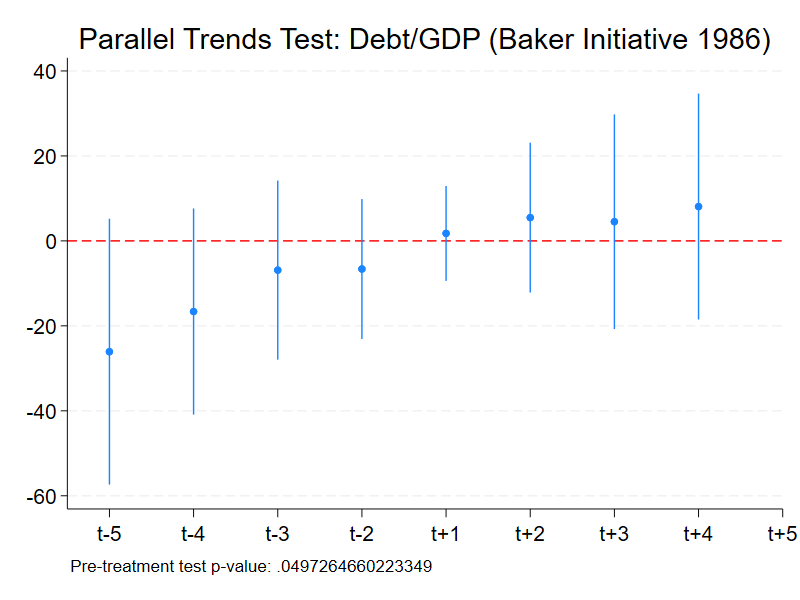
\includegraphics[width=\textwidth]{figures/PT_Baker_Debt.png}
        \caption{Parallel Trend Test 1}
        \label{fig:pt1_eme}
    \end{subfigure}
    \hfill
    \begin{subfigure}[b]{0.48\textwidth}
        \centering
        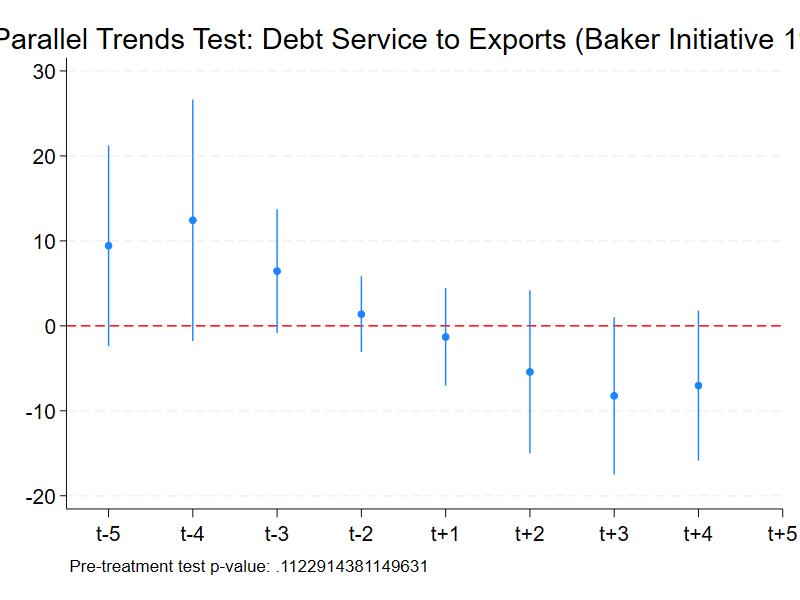
\includegraphics[width=\textwidth]{figures/PT_Baker_DebtServ.png}
        \caption{Parallel Trend Test 2}
        \label{fig:pt2_eme}
    \end{subfigure}
    \\[1em]
    \begin{subfigure}[b]{0.48\textwidth}
        \centering
        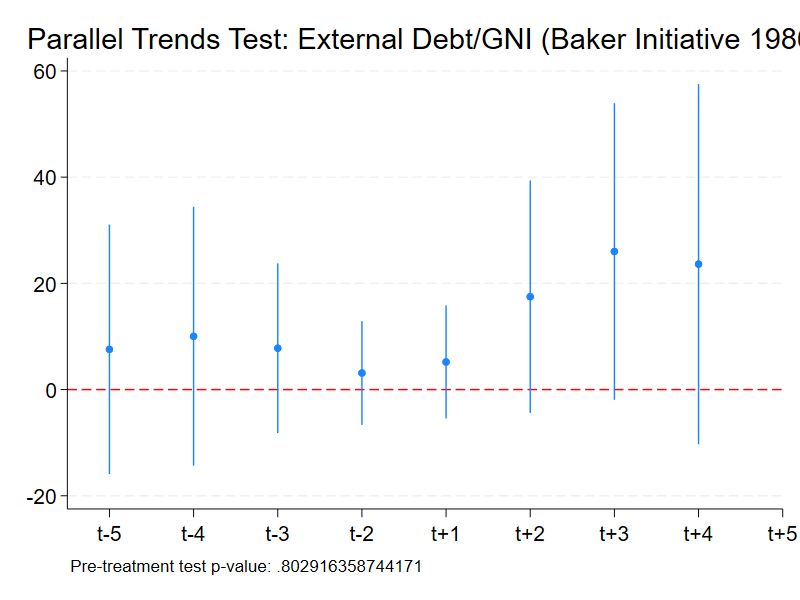
\includegraphics[width=\textwidth]{figures/PT_Baker_ExtDebt.png}
        \caption{Parallel Trend Test 3}
        \label{fig:pt3_eme}
    \end{subfigure}
    \hfill
    \begin{subfigure}[b]{0.48\textwidth}
        \centering
        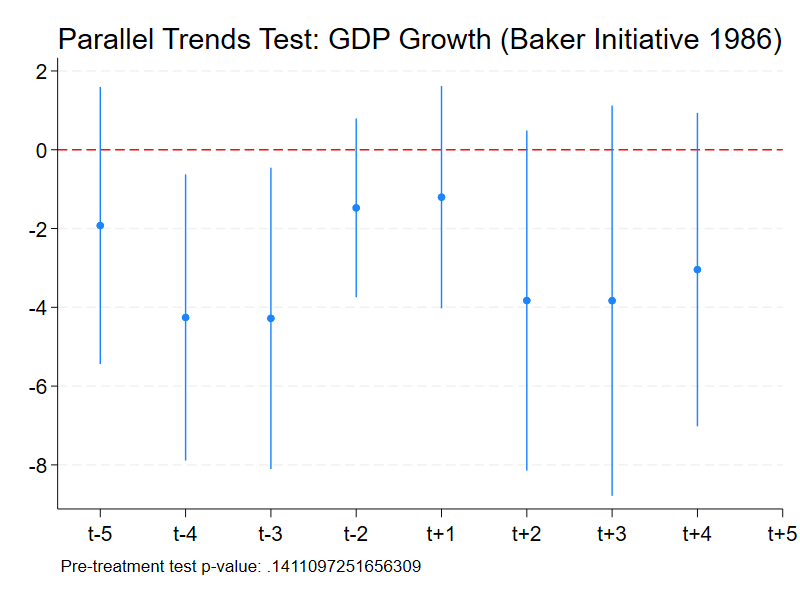
\includegraphics[width=\textwidth]{figures/PT_Baker_GDP.png}
        \caption{Parallel Trend Test 4}
        \label{fig:pt4_eme}
    \end{subfigure}
    \\[1em]
    \begin{subfigure}[b]{0.48\textwidth}
        \centering
        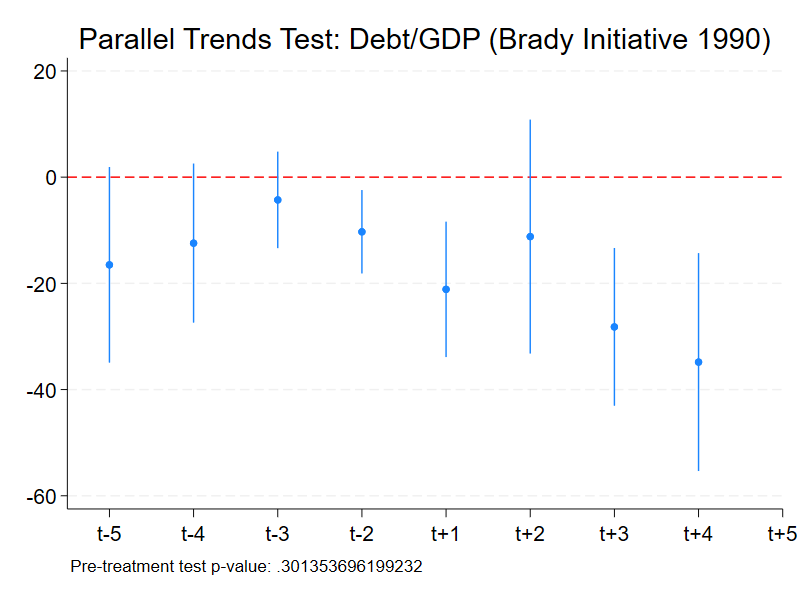
\includegraphics[width=\textwidth]{figures/PT_Brady_Debt.png}
        \caption{Parallel Trend Test 5}
        \label{fig:pt5_eme}
    \end{subfigure}
    \hfill
    \begin{subfigure}[b]{0.48\textwidth}
        \centering
        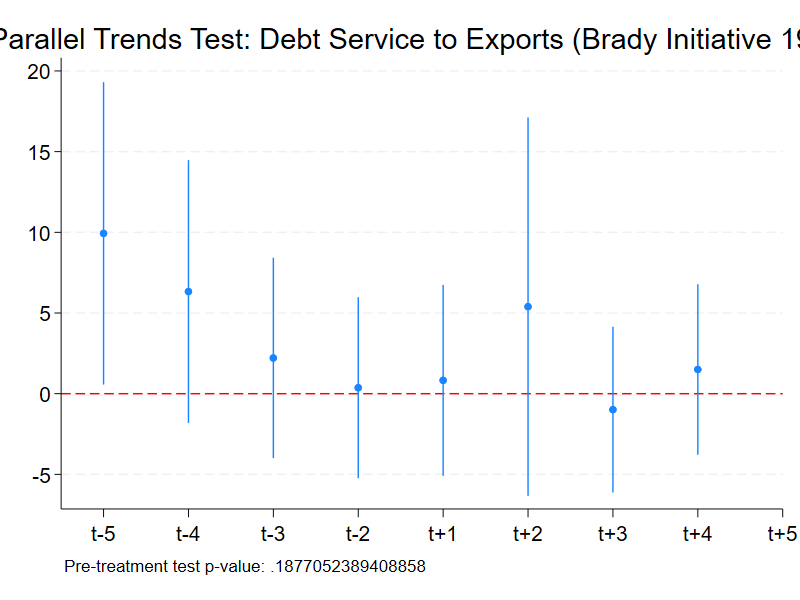
\includegraphics[width=\textwidth]{figures/PT_Brady_DebtServ.png}
        \caption{Parallel Trend Test 6}
        \label{fig:pt6_eme}
    \end{subfigure}
    \\[1em]
    \begin{subfigure}[b]{0.48\textwidth}
        \centering
        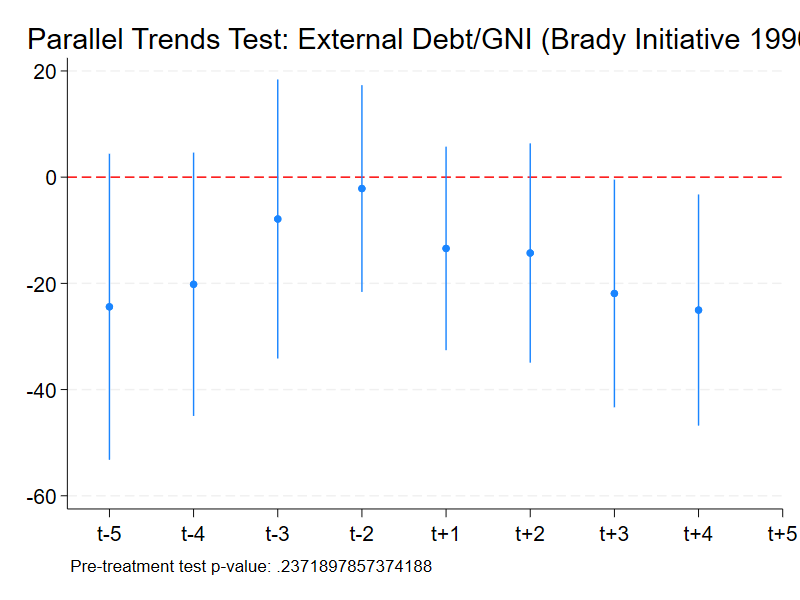
\includegraphics[width=\textwidth]{figures/PT_Brady_ExtDebt.png}
        \caption{Parallel Trend Test 7}
        \label{fig:pt7_eme}
    \end{subfigure}
    \hfill
    \begin{subfigure}[b]{0.48\textwidth}
        \centering
        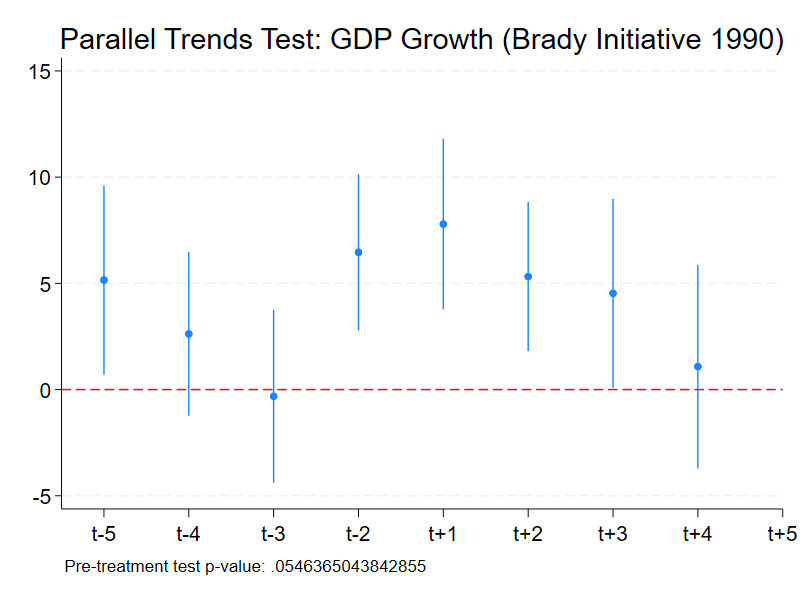
\includegraphics[width=\textwidth]{figures/PT_Brady_GDP.png}
        \caption{Parallel Trend Test 8}
        \label{fig:pt8_eme}
    \end{subfigure}
    \caption{Parallel trend test results for EME case}
    \label{fig:parallel_trends3}
\end{figure}

\begin{figure}[ht!]
    \centering
    \begin{subfigure}[b]{0.48\textwidth}
        \centering
        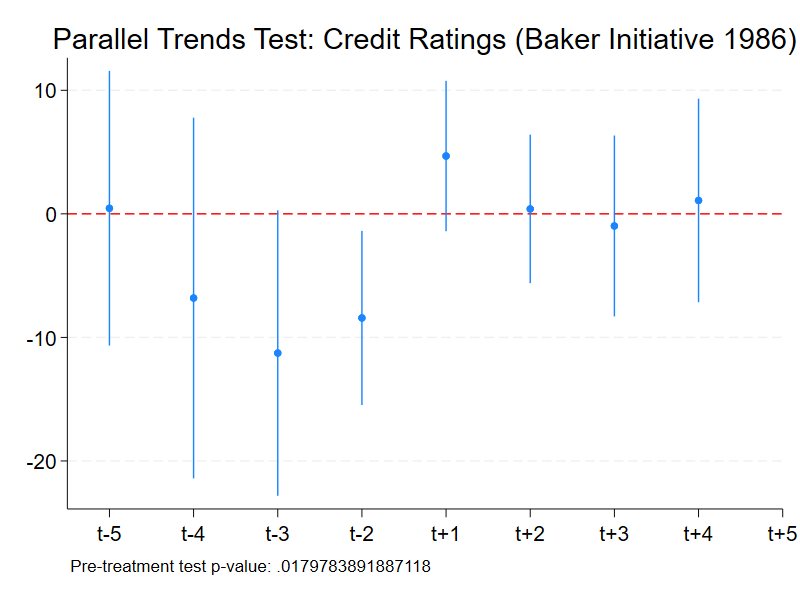
\includegraphics[width=\textwidth]{figures/PT_Baker_Ratings.png}
        \caption{Parallel Trend Test 9}
        \label{fig:pt9_eme}
    \end{subfigure}
    \hfill
    \begin{subfigure}[b]{0.48\textwidth}
        \centering
        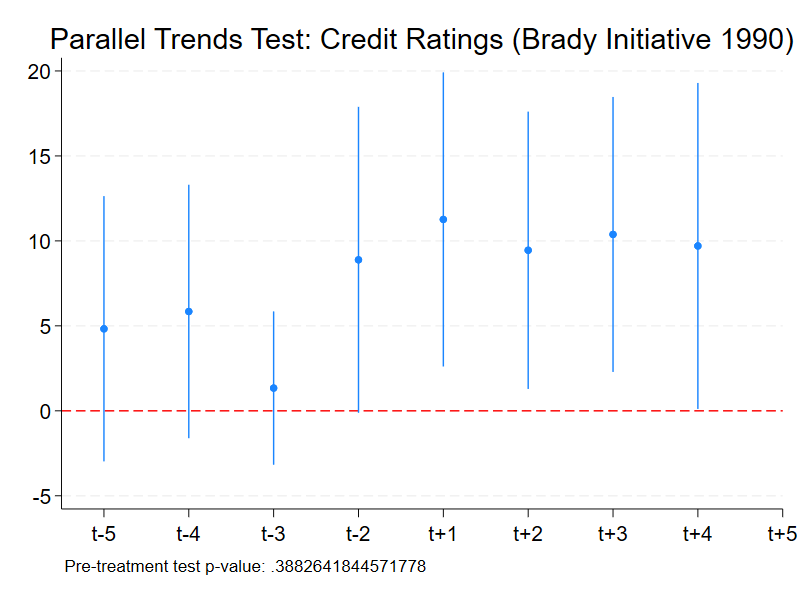
\includegraphics[width=\textwidth]{figures/PT_Brady_Ratings.png}
        \caption{Parallel Trend Test 10}
        \label{fig:pt10_eme}
    \end{subfigure}
    \caption{Parallel trend test results for EME case}
    \label{fig:parallel_trends4}
\end{figure}

In Table 5,
the treatment coefficient for output growth is negative and insignificant for the Baker
episode. Also, debt/GDP continues to grow post-treatment. On the positive side, we
find evidence that the credit ratings of the Baker countries increase significantly more
than the counterfactual (also because the time window includes the 1990/1991 Brady
years). Moreover, the treatment coefficient for debt servicing is negative and marginally
significant, indicating that the Baker plan indeed brought cash flow relief.

\begin{table}[ht!]\centering
\def\sym#1{\ifmmode^{#1}\else\(^{#1}\)\fi}
\caption{Table 5: Baker Initiative (1986) - Difference-in-Difference Analysis}
\renewcommand{\arraystretch}{1.2} % 增加行距
\begin{tabular*}{\textwidth}{@{\hskip\tabcolsep\extracolsep\fill}p{4cm}*{5}{>{\centering\arraybackslash}p{2cm}}}
\hline\hline
            &(1)&(2)&(3)&(4)&(5)\\
            &\parbox{2cm}{\centering Growth, real p.c.}&\parbox{2cm}{\centering Credit Ratings (change)}&\parbox{2cm}{\centering Debt Service to Exports}&\parbox{2cm}{\centering Total Public Debt/GDP}&\parbox{2cm}{\centering External Debt/GNI}\\
\hline
\parbox{4cm}{\raggedright Post-1986 dummy}&  $-1.976$  &  $-5.968^{**}$  &  $-5.758$  &  $-17.214^{**}$  &  $-8.881$  \\
            &  $(1.292)$  &  $(2.328)$ & $(3.426)$   &  $(7.106)$   &  $(6.251)$  \\
[0.5em]
\parbox{4cm}{\raggedright Baker Treatment $\times$ Post-1986}&  $-1.918$&  $6.305^{*}$  &  $-9.049^{*}$&  $22.988^{**}$  &  $17.432$   \\
            &  $(1.329)$   &  $(3.121)$   &  $(4.720)$   &  $(9.360)$   &  $(10.802)$   \\
\hline
Observations&       $275$   &       $279$   &       $189$   &       $226$   &       $199$   \\
R-squared   &       $0.111$   &       $0.200$   &       $0.154$   &       $0.238$   &       $0.189$   \\
Adjusted R² &       $0.077$   &       $0.170$   &       $0.106$   &       $0.203$   &       $0.145$   \\
\hline\hline
\multicolumn{6}{p{0.95\textwidth}}{\footnotesize \textbf{Notes:} This table reports difference-in-difference estimates of the effect of the Baker Initiative on various economic outcomes. Treatment group consists of countries that received Baker Plan debt relief. All regressions include country and year fixed effects. Time window: 1981-1990 (5 years before and after 1986). Standard errors clustered at country level in parentheses. $^*$ p<0.10, $^{**}$ p<0.05, $^{***}$ p<0.01}\\
\end{tabular*}
\end{table}


\begin{table}[ht!]\centering
\def\sym#1{\ifmmode^{#1}\else\(^{#1}\)\fi}
\caption{Table 6: Brady Initiative (1990) - Difference-in-Difference Analysis}
\renewcommand{\arraystretch}{1.2} % 增加行距
\begin{tabular*}{\textwidth}{@{\hskip\tabcolsep\extracolsep\fill}p{4cm}*{5}{>{\centering\arraybackslash}p{2cm}}}
\hline\hline
            &(1)&(2)&(3)&(4)&(5)\\
            &\parbox{2cm}{\centering Growth, real p.c.}&\parbox{2cm}{\centering Credit Ratings (change)}&\parbox{2cm}{\centering Debt Service to Exports}&\parbox{2cm}{\centering Total Public Debt/GDP}&\parbox{2cm}{\centering External Debt/GNI}\\
\hline
\parbox{4cm}{\raggedright Post-1990 dummy}&  $1.207$  &  $5.061^*$  &  $-1.884$  &  $-15.324^{**}$  &  $-10.819$  \\
            &  $(1.350)$  &  $(2.505)$ & $(2.461)$   &  $(7.101)$   &  $(9.069)$  \\
[0.5em]
\parbox{4cm}{\raggedright Brady Treatment $\times$ Post-1990}&  $3.094^{***}$&  $6.991^{**}$  &  $-1.565$&  $-14.514^*$  &  $-1.821$   \\
            &  $(1.046)$   &  $(3.095)$   &  $(3.542)$   &  $(7.377)$   &  $(10.677)$   \\
\hline
Observations&       $270$   &       $270$   &       $190$   &       $233$   &       $200$   \\
R-squared   &       $0.132$   &       $0.242$   &       $0.299$   &       $0.275$   &       $0.089$   \\
Adjusted R² &       $0.099$   &       $0.213$   &       $0.259$   &       $0.242$   &       $0.041$   \\
\hline\hline
\multicolumn{6}{p{0.95\textwidth}}{\footnotesize \textbf{Notes:} This table reports difference-in-difference estimates of the effect of the Brady Initiative on various economic outcomes. Treatment group consists of countries that received Brady Plan debt relief. All regressions include country and year fixed effects. Time window: 1986-1995 (5 years before and after 1990). Standard errors clustered at country level in parentheses. $^*$ p<0.10, $^{**}$ p<0.05, $^{***}$ p<0.01}\\
\end{tabular*}
\end{table}


The most notable change between the Baker and Brady regression results (Tables 5
and 6) is in column (1). The treatment coefficient for real per capita GDP growth turns
positive and highly significant, indicating that the Brady debt relief operation translated
into 3 percentage point higher growth, compared to the counterfactual of non-crisis
emerging markets. This is a sizable coefficient, which resembles that of the 1934
episode (Table 4). Also, the credit ratings of Brady countries see a large improvement
relative to the counterfactual (of 7 IIR index points, on average), while government
debt levels drop significantly more (by 15 percentage points). Surprisingly, however,
we find no significant effect on debt servicing or for total external debt/GDP, possibly
because the actual Brady restructurings took place with a lag in many countries, as
discussed previously.



\section{Staggered DiD Analysis}
According to the author, the Brady Plan was actually implemented in a staggered
fashion, with some countries starting in 1989 and others following until 1995.

To account for this, we use the Callaway-Sant'Anna (2021) staggered difference-in-differences
(CSDID) estimator, which allows for heterogeneous treatment effects and
dynamic treatment effects over time.

\begin{figure}[ht!]
    \centering
    \begin{subfigure}[b]{0.48\textwidth}
        \centering
        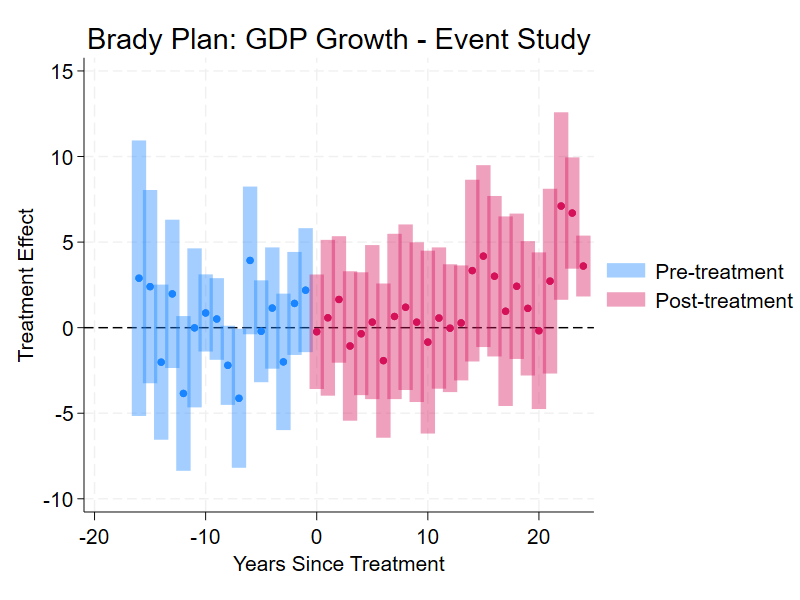
\includegraphics[width=\textwidth]{figures/CS_Brady_Growth_EventStudy.png}
        \caption{Staggered DiD Result 1}
        \label{fig:stag1}
    \end{subfigure}
    \hfill
    \begin{subfigure}[b]{0.48\textwidth}
        \centering
        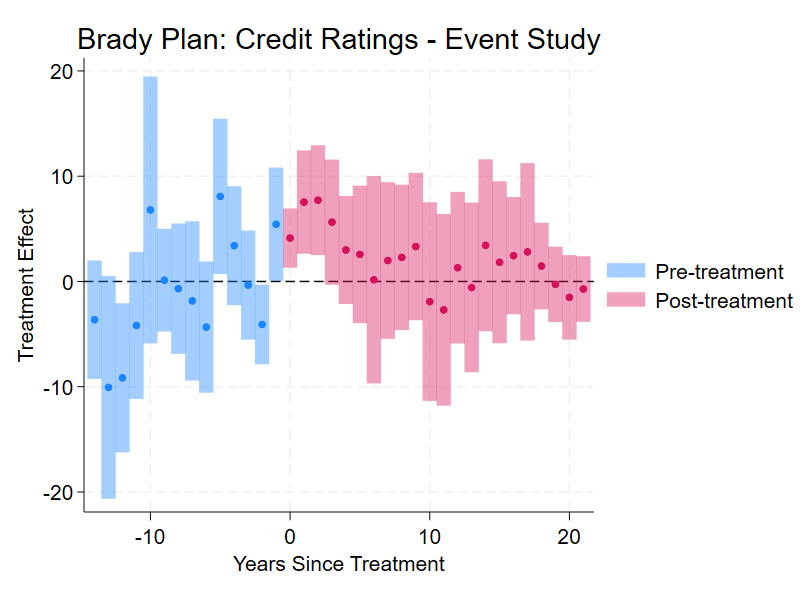
\includegraphics[width=\textwidth]{figures/CS_Brady_Ratings_EventStudy.png}
        \caption{Staggered DiD Result 2}
        \label{fig:stag2}
    \end{subfigure}
    \\[1em]
    \begin{subfigure}[b]{0.48\textwidth}
        \centering
        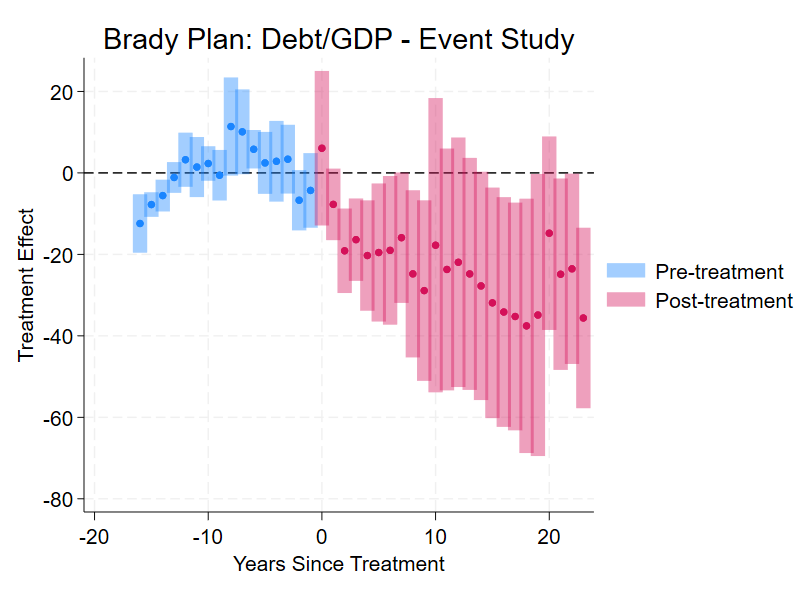
\includegraphics[width=\textwidth]{figures/CS_Brady_Debt_EventStudy.png}
        \caption{Staggered DiD Result 3}
        \label{fig:stag3}
    \end{subfigure}
    \hfill
    \begin{subfigure}[b]{0.48\textwidth}
        \centering
        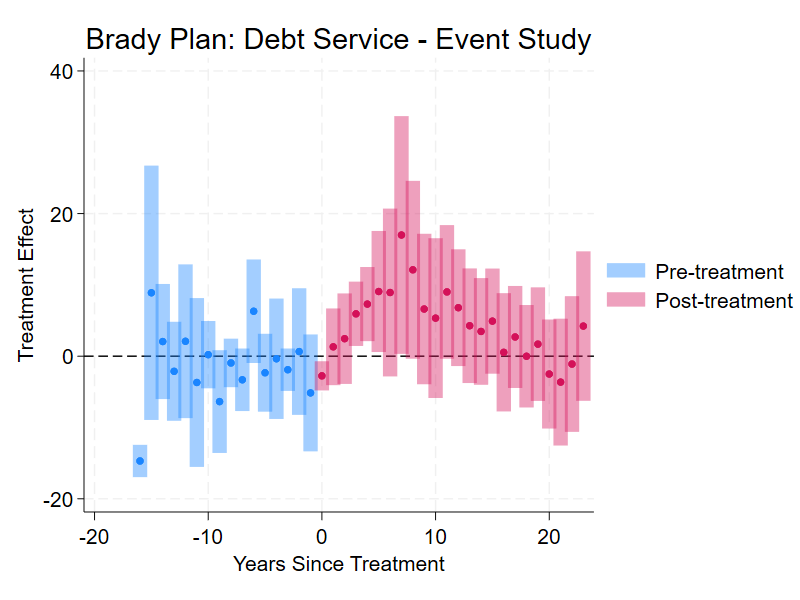
\includegraphics[width=\textwidth]{figures/CS_Brady_DebtService_EventStudy.png}
        \caption{Staggered DiD Result 4}
        \label{fig:stag4}
    \end{subfigure}
    \\[1em]
    \begin{subfigure}[b]{0.48\textwidth}
        \centering
        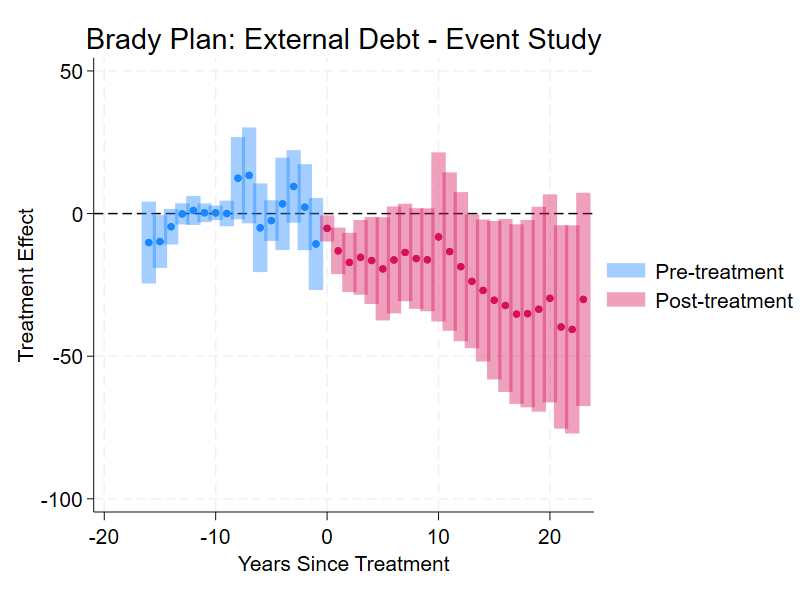
\includegraphics[width=\textwidth]{figures/CS_Brady_ExtDebt_EventStudy.png}
        \caption{Staggered DiD Result 5}
        \label{fig:stag5}
    \end{subfigure}
    \caption{Staggered Difference-in-Differences Analysis Results}
    \label{fig:staggered_did}
\end{figure}

To see it in a more clear way, we also write the results into a table:

\begin{table}[ht!]\centering
\def\sym#1{\ifmmode^{#1}\else\(^{#1}\)\fi}
\caption{Brady Plan (1989-1995) - Callaway-Sant'Anna Staggered Difference-in-Differences Analysis}
\renewcommand{\arraystretch}{1.2} % 增加行距
\begin{tabular*}{\textwidth}{@{\hskip\tabcolsep\extracolsep\fill}p{4cm}*{5}{>{\centering\arraybackslash}p{2cm}}}
\hline\hline
            &(1)&(2)&(3)&(4)&(5)\\
            &\parbox{2cm}{\centering Growth, real p.c.}&\parbox{2cm}{\centering Credit Ratings (change)}&\parbox{2cm}{\centering Debt Service to Exports}&\parbox{2cm}{\centering Total Public Debt/GDP}&\parbox{2cm}{\centering External Debt/GNI}\\
\hline
\parbox{4cm}{\raggedright Average Treatment Effect on Treated (ATT)}&  $1.005$  &  $2.331$  &  $5.047$  &  $-22.587^{**}$  &  $-20.799^{**}$  \\
            &  $(1.923)$  &  $(2.494)$ & $(3.299)$   &  $(9.722)$   &  $(9.550)$  \\
[0.5em]
\hline
Treatment Countries&       $16$   &       $16$   &       $16$   &       $16$   &       $16$   \\
Control Countries   &       $24$   &       $24$   &       $24$   &       $24$   &       $24$   \\
% Treatment Period     &       \multicolumn{5}{c}{$1989-1995$}   \\
% Method              &       \multicolumn{5}{c}{Callaway-Sant'Anna (2021)}   \\
\hline\hline
\multicolumn{6}{p{0.95\textwidth}}{\footnotesize \textbf{Notes:} This table presents average treatment effects on the treated (ATT) from the Callaway and Sant'Anna (2021) staggered difference-in-differences estimator using actual Brady Plan implementation dates by country. Treatment timing varies from 1989-1995: Mexico, Philippines, Costa Rica (1989); Uruguay, Venezuela (1990); Nigeria (1991); Argentina, Brazil (1992); Bolivia, Bulgaria, Dominican Republic, Jordan (1993); Ecuador, Poland (1994); Panama, Peru (1995). Control group consists of emerging market economies that never implemented Brady agreements. The method accounts for treatment effect heterogeneity across cohorts and time periods using doubly robust inverse probability weighting (DRIPW). Standard errors clustered at country level in parentheses. $^*$ p<0.10, $^{**}$ p<0.05, $^{***}$ p<0.01}\\
\end{tabular*}
\end{table}


\begin{enumerate}[label=(\arabic*),leftmargin=1.25cm]
    \item \textbf{Real per-capita GDP growth}.  
    The point estimate of \(\text{ATT}=1.005\) (s.e.\;1.923) is economically small and statistically insignificant.\footnote{All hypothesis tests use two-sided $t$-statistics with 39 degrees of freedom.}  
    Hence, short-run output gains attributable solely to the Brady restructuring appear limited.

    \item \textbf{Credit-rating upgrades}.  
    The estimated improvement of \(2.331\) notches (s.e.\;2.494) is likewise imprecisely measured, suggesting that sovereign creditworthiness did not accelerate immediately after restructuring.

    \item \textbf{Debt-service pressure}.  
    The debt-service-to-exports ratio rises by \(5.047\) percentage points (s.e.\;3.299) but remains insignificant.  
    A mechanical uptick is plausible because coupon payments on the new Brady bonds were front-loaded, even though principal obligations were reduced.

    \item \textbf{Public-debt burden}.  
    A statistically significant fall of \(-22.587^{**}\) percentage points of GDP (s.e.\;9.722) confirms that the Brady exchanges achieved their primary aim: \emph{a sizable reduction in public debt stocks}.

    \item \textbf{External indebtedness}.  
    External debt drops by \(-20.799^{**}\) percentage points of GNI (s.e.\;9.550).  
    The comparable magnitude across the two debt ratios underscores that the relief was broad-based, not merely an accounting reshuffle between domestic and foreign holders.
\end{enumerate}

\paragraph{Methodological strengths.}
The staggered estimator weights cohort-specific counterfactuals, eliminating negative-weight bias inherent in traditional two-way fixed effects when treatment timing is staggered.  
Doubly robust inverse-probability weighting (DRIPW) further guards against misspecification in both the propensity-score and outcome equations, enhancing credibility.

\paragraph{Economic implications.}
\begin{itemize}[leftmargin=0.9cm]
    \item \emph{Debt relief first, growth later.}  The significant contraction in debt ratios signals successful balance-sheet repair.  However, growth dividends are not immediate; structural reforms and a longer horizon may be required for debt relief to translate into higher output.
    \item \emph{Market sentiment lags policy action.}  Credit-rating agencies reacted cautiously, consistent with historical evidence that ratings improve only after sustained fiscal consolidation.
    \item \emph{Policy design.}  Future restructurings should pair liability management with complementary reforms (e.g.\ trade liberalisation, financial-sector deepening) to accelerate real-sector recovery.
\end{itemize}

\paragraph{Limitations.}
The evaluation window (1989-1995) captures only the first six years after each country's exchange.  If growth effects materialise with longer lags, the present estimates are lower bounds.  Moreover, macro-shocks in the early 1990s (e.g.\ the Tequila crisis) may attenuate observed treatment effects despite the DiD controls.
